\documentclass[12pt]{article}

% ============================================================
% PACKAGES
% ============================================================

\usepackage{amsmath}
\usepackage{amssymb}
\usepackage{amsthm}
\usepackage{mathtools}
\usepackage{bm}

\usepackage{booktabs}
\usepackage{threeparttable}
\usepackage{multirow}
\usepackage{array}
\usepackage{graphicx}
\usepackage{adjustbox}
\usepackage{placeins}
\usepackage{float}
\usepackage{subcaption}

\usepackage[margin=1in]{geometry}
\usepackage{setspace}
\onehalfspacing

\usepackage[authoryear,round]{natbib}

\usepackage[
    colorlinks=true,
    citecolor=blue,
    linkcolor=blue,
    urlcolor=blue
]{hyperref}

\usepackage{enumitem}
\usepackage{xcolor}
\usepackage{microtype}

% ============================================================
% THEOREM ENVIRONMENTS
% ============================================================

\newtheorem{proposition}{Proposition}
\newtheorem{lemma}{Lemma}
\newtheorem{corollary}{Corollary}
\newtheorem{assumption}{Assumption}

\theoremstyle{definition}
\newtheorem{definition}{Definition}

\theoremstyle{remark}
\newtheorem{remark}{Remark}

% ============================================================
% CUSTOM COMMANDS
% ============================================================

\newcommand{\E}{\mathbb{E}}
\newcommand{\Var}{\operatorname{Var}}
\newcommand{\Cov}{\operatorname{Cov}}
\newcommand{\Prob}{\mathbb{P}}

\newcommand{\argmax}{\operatorname*{arg\,max}}
\newcommand{\argmin}{\operatorname*{arg\,min}}

% ============================================================
% TITLE
% ============================================================

\title{Dynamic Optimal Pricing with Preferences for Novelty}
\author{Tate Mason}
\date{\today}

% ============================================================
% DOCUMENT
% ============================================================

\begin{document}

\maketitle

\begin{abstract}
  INSERT ABSTRACT
\end{abstract}

\newpage

% ============================================================
% INTRODUCTION
% ============================================================

\section{Introduction}
\label{sec:introduction}

As shopping becomes an increasingly online endeavor, firms are privy to ever-increasing information on their consumers. Algorithmic recommendations, personalized feeds, and personalized discounts are all common practice by firms to entice consumers to purchase their product. One type of data the firm could employ to target consumers is how their consumption varies with time. An example of this behavior is personalized coupons from a grocery store. Using these coupons, the firm could feasibly steer consumers towards certain products through bundling or discounting. This paper seeks to understand how valuable consumers' purchase histories are for personalized pricing when consumers differ in their preferences for novelty and habit?

I examine the value of information on consumer types by solving a two-period theoretical model for optimal pricing and profit. Then, using Nielsen HomeScan and MarketScan data, I estimate the distribution of preferences for novelty, habit, and price sensitivity for consumers. I then map my empirical results to the theoretical to examine the efficacy of targeted couponing for the firm. The firm can observe consumption histories and preferences for novelty to target. I then compare revenues in the full infomation case to one in which the firm has obscured information on consumer types.

In the theoretical exercise, I see distinct pricing patterns depending on consumer type and histories. For high switching types, the firm must calculate the continuation-value tradeoff, deciding if reduced early profit is worth later profit. In the case of high switchers, the firm will charge high prices in period one, knowing the likelihood of switching away is high. For consumers who habitually consume the same good, the firm will go so far as to subsidize the outside good consumer to induce switching while charging a higher price to those who start inside, knowing they will likely stay on their product. 

Empirically, I find that consumers do not like novelty, incurring disutility equivalent to \$2.07. Consumers gain slight utility from habitual consuption, preferring to have a high percentage of total consumption be their preferred good. However, there is substantial heterogeneity in these tastes. When applying the estimated distribution of novelty to the supply exercise, I find the firm yields simulated gains in revenue when doing targeted disconuting. This can be up to 12\% versus the no-coupon case.


% ============================================================
% BACKGROUND AND LITERATURE
% ============================================================

\section{Related Literature and Contribution}
\label{sec:literature}

SUPPLY LITERATURE - TARGETED PRICING AND STATE DEPENDENCE
DEMAND LITERATURE - ESTIMATION OF PREFERENCES AND MODELING

CONTRIBUTION - TYPE DISTRIBUTION, FIRM PRICING OFF TYPE



% ============================================================
% THEORETICAL SUPPLY SIDE
% ============================================================

\section{Theoretical Framework}
\label{sec:theory}
% Mathematical update follows supply_code/MODEL_CONVENTIONS.md and
% supply_code/comparative_statics/canonical.py (symmetric switching).
% Superseded prose and equations are preserved in supply_previous.tex.

\subsection{Consumer Demand}
\label{subsec:model-demand}
In each period $t\in\{1,2\}$, the consumer chooses the inside good $j$ or
outside good $0$. Let $h=x_{t-1}\in\{j,0\}$ denote the previous choice.
For a fixed switching type $r$, deterministic utilities are
\begin{align}
 V_{jt}^{\mathrm{inside}}(h)
 &=\underbrace{\beta}_{\text{Baseline utility}}
 +\underbrace{\gamma_r\mathbf{1}\{h=0\}}_{\text{Utility from switching}}
 +\underbrace{\alpha p_t(h)}_{\text{Price disutility}},\\
 V_{0t}^{\mathrm{outside}}(h)
 &=\gamma_r\mathbf{1}\{h=j\}.
\end{align}
Here $\alpha<0$. Subtracting outside utility gives
\begin{align}
 v_t(h)&=V_{jt}^{\mathrm{inside}}(h)-V_{0t}^{\mathrm{outside}}(h)\notag\\
 &=\beta+\gamma_r\bigl[\mathbf{1}\{h=0\}-\mathbf{1}\{h=j\}\bigr]
 +\alpha p_t(h).
\end{align}
Define the signed history indicator
\begin{equation}
 q(h)=\mathbf{1}\{h=0\}-\mathbf{1}\{h=j\}
 =\begin{cases}
  1,&h=0,\\
  -1,&h=j.
 \end{cases}
\end{equation}
Suppressing the fixed type subscript from here onward,
\begin{equation}
 v_t(h)=\beta+q(h)\gamma+\alpha p_t(h).
\end{equation}
With independent Type-I extreme-value shocks on both alternatives, choice shares are
\begin{align}
 s_t(h)&=\frac{e^{v_t(h)}}{1+e^{v_t(h)}},
 \label{eq:supply-share}\\
 s_{0t}(h)&=1-s_t(h).
\end{align}

\subsection{Firm's Problem}
\label{subsec:firm-problem}
Let $h=x_0$ be the initial choice and $a=x_1$ the realized first-period choice.
All profits below are per consumer, conditional on the firm-observed type and initial state.
Marginal cost $c$ is fixed, $0<\delta<1$, and prices are unrestricted real numbers.
\begin{align}
 W_2(a)&=\max_{p_2(a)\in\mathbb R}s_2(a)[p_2(a)-c],
 \qquad \Delta W=W_2(j)-W_2(0),\\
 \Pi(p_1;h)&=s_1(h)(p_1-c)
 +\delta\{s_1(h)W_2(j)+[1-s_1(h)]W_2(0)\}\notag\\
 &=\delta W_2(0)+s_1(h)[p_1-c+\delta\Delta W],
 \label{eq:supply-profit}\\
 \Pi^*(h)&=\max_{p_1(h)\in\mathbb R}\Pi(p_1;h).
\end{align}
For initial-state probabilities $\mu_r(h)$ and type populations $N_r$,
\begin{equation}
 \Pi_{\mathrm{total}}^*=\sum_r N_r\sum_{h\in\{j,0\}}\mu_r(h)\Pi_r^*(h),
 \qquad \sum_h\mu_r(h)=1.
\end{equation}

\section{Optimal Pricing}
\label{sec:optimal-pricing}
A star denotes an optimized price or share. For the comparative statics below, write
\begin{align*}
 s&=s_1^*(h), & \ell&=1-s,\\
 u&=s_2^*(j), & v&=s_2^*(0),\\
 B&=u+v.
\end{align*}

\subsection{Period Two}
\label{subsec:foc}
For each realized first-period choice $a\in\{j,0\}$,
\begin{align}
 0&=s_2+\alpha s_2(1-s_2)(p_2-c),\\
 p_2^*(a)&=c-\frac{1}{\alpha[1-s_2^*(a)]}.
 \label{eq:supply-terminal}
\end{align}
The corresponding continuation value is
\begin{equation}
 W_2(a)=-\frac{s_2^*(a)}{\alpha[1-s_2^*(a)]}.
\end{equation}

\subsection{Period One}
\label{subsec:price-derivation}
With $\Delta W=W_2(j)-W_2(0)$,
\begin{align}
 0&=s_1+\alpha s_1(1-s_1)[p_1-c+\delta\Delta W],\\
 p_1^*(h)&=c-\frac{1}{\alpha\ell}-\delta\Delta W.
 \label{eq:supply-first}
\end{align}
Expected profit at the optimum is
\begin{equation}
 \Pi^*(h)=\delta W_2(0)-\frac{s}{\alpha\ell}.
\end{equation}
Shares in these implicit pricing equations are evaluated at the optimal prices.
Full derivations are in Appendix~\ref{app:supply}.

\subsection{Static Benchmark}
The static counterfactual is solved separately:
\begin{align}
 p^{\mathrm{stat}}(h)&=c-\frac{1}{\alpha[1-s^{\mathrm{stat}}(h)]},\\
 s^{\mathrm{stat}}(h)&=\frac{e^{\beta+\alpha p^{\mathrm{stat}}(h)+q(h)\gamma}}
 {1+e^{\beta+\alpha p^{\mathrm{stat}}(h)+q(h)\gamma}}.
\end{align}

\section{Comparative Statics}
\label{sec:comparative-statics}
All derivatives hold the discrete history and other parameters fixed and allow
optimal prices to respond.

\subsection{Switching Preferences: Prices}
\begin{align}
 \frac{dp_2^*(a)}{d\gamma}&=-\frac{q(a)s_2^*(a)}{\alpha},\\
 \frac{dp_1^*(h)}{d\gamma}&=-\frac{q(h)s+\delta\ell(u+v)}{\alpha}.
 \label{eq:supply-gamma-prices}
\end{align}
The terminal-price signs are
\begin{equation}
 \frac{dp_2^*(j)}{d\gamma}<0,\qquad
 \frac{dp_2^*(0)}{d\gamma}>0.
\end{equation}
For first-period prices,
\begin{align}
 \frac{dp_1^*(0)}{d\gamma}&>0,\\
 \frac{dp_1^*(j)}{d\gamma}>0
 &\iff\delta\ell(u+v)>s.
\end{align}

\subsection{Switching Preferences: Profit}
\begin{equation}
 \frac{d\Pi^*(h)}{d\gamma}
 =\frac{-q(h)s+\delta(su-\ell v)}{\alpha}.
 \label{eq:supply-gamma-profit}
\end{equation}
The signs depend on the initial state:
\begin{align}
 \frac{d\Pi^*(0)}{d\gamma}&>0,\\
 \frac{d\Pi^*(j)}{d\gamma}>0
 &\iff\delta\ell v>s(1+\delta u).
\end{align}

\subsection{Discount Factor}
\begin{align}
 \frac{dp_2^*(a)}{d\delta}&=0,\\
 \frac{dp_1^*(h)}{d\delta}&=-\ell\Delta W.
\end{align}
Since $\Delta W$ has the opposite sign to $\gamma$,
\begin{equation}
 \operatorname{sgn}\!\left(\frac{dp_1^*(h)}{d\delta}\right)
 =\operatorname{sgn}(\gamma).
\end{equation}
At $\gamma=0$, the continuation values coincide and
$p_1^*(h)=p^{\mathrm{stat}}(h)$.

\subsection{Baseline Utility}
\begin{align}
 \frac{dp_2^*(a)}{d\beta}&=-\frac{s_2^*(a)}{\alpha},\\
 \frac{dp_1^*(h)}{d\beta}&=\frac{-s+\delta\ell(u-v)}{\alpha}.
\end{align}
Thus
\begin{equation}
 \frac{dp_1^*(h)}{d\beta}>0\iff s>\delta\ell(u-v).
\end{equation}

\subsection{Price Sensitivity}
\begin{align}
 \frac{dp_2^*(a)}{d\alpha}&=\frac{1}{\alpha^2}
 -\frac{s_2^*(a)p_2^*(a)}{\alpha},\\
 \frac{dp_1^*(h)}{d\alpha}&=\frac{1}{\alpha^2}
 -\frac{sp_1^*(h)}{\alpha}
 +\frac{\delta\ell}{\alpha}[up_2^*(j)-vp_2^*(0)].
\end{align}
For the positive measure of price sensitivity $-\alpha$,
\begin{equation}
 \frac{dp_t^*}{d(-\alpha)}=-\frac{dp_t^*}{d\alpha}.
\end{equation}

\subsection{Price Ratios}
For each $(h,a)\in\{(0,0),(0,j),(j,j),(j,0)\}$ with $p_2^*(a)\ne0$,
\begin{align}
 R_{h,a}&=\frac{p_1^*(h)}{p_2^*(a)},\\
 \frac{dR_{h,a}}{d\gamma}
 &=\frac{p_2^*(a)\,dp_1^*(h)/d\gamma
 -p_1^*(h)\,dp_2^*(a)/d\gamma}{[p_2^*(a)]^2}.
\end{align}

\subsection{Profit Conditional on the First-Period Choice}
\begin{align}
 \Pi^*(h,a)&=\mathbf{1}\{a=j\}[p_1^*(h)-c]+\delta W_2(a),\\
 \Pi^*(h)&=s\Pi^*(h,j)+\ell\Pi^*(h,0).
\end{align}

\subsection{Numerical Supply Results}
\begin{equation*}
 \beta=2,\qquad\alpha=-1,\qquad\delta=0.92,\qquad c=0,
 \qquad\gamma\in[-3,3].
\end{equation*}
\begin{table}[htbp]
\centering\small
\caption{Selected optimal prices and profits in the theoretical supply model}
\label{tab:supply-solutions}
\begin{tabular}{crrrrrr}\toprule
  $x_0$ & $\gamma$ & $p_1^*$ & $p_2^*(j)$ & $p_2^*(0)$ & $\Pi^*$ & $\Pi^{*\prime}$\\\midrule
  $j$ & -3 & 3.395 & 3.926 & 1.120 & 5.087 & -1.387\\
  $j$ & -1 & 2.236 & 2.557 & 1.567 & 2.669 & -0.959\\
  $j$ & 0 & 2.000 & 2.000 & 2.000 & 1.920 & -0.500\\
  $j$ & 1 & 2.209 & 1.567 & 2.557 & 1.731 & 0.125\\
  $j$ & 3 & 3.592 & 1.120 & 3.926 & 2.702 & 0.668\\
  $0$ & -3 & -0.780 & 3.926 & 1.120 & 0.913 & 0.195\\
  $0$ & -1 & 1.045 & 2.557 & 1.567 & 1.478 & 0.385\\
  $0$ & 0 & 2.000 & 2.000 & 2.000 & 1.920 & 0.500\\
  $0$ & 1 & 2.956 & 1.567 & 2.557 & 2.478 & 0.615\\
  $0$ & 3 & 4.801 & 1.120 & 3.926 & 3.912 & 0.804\\
  \bottomrule\end{tabular}
\end{table}
\FloatBarrier
\begin{figure}[htbp]
\centering
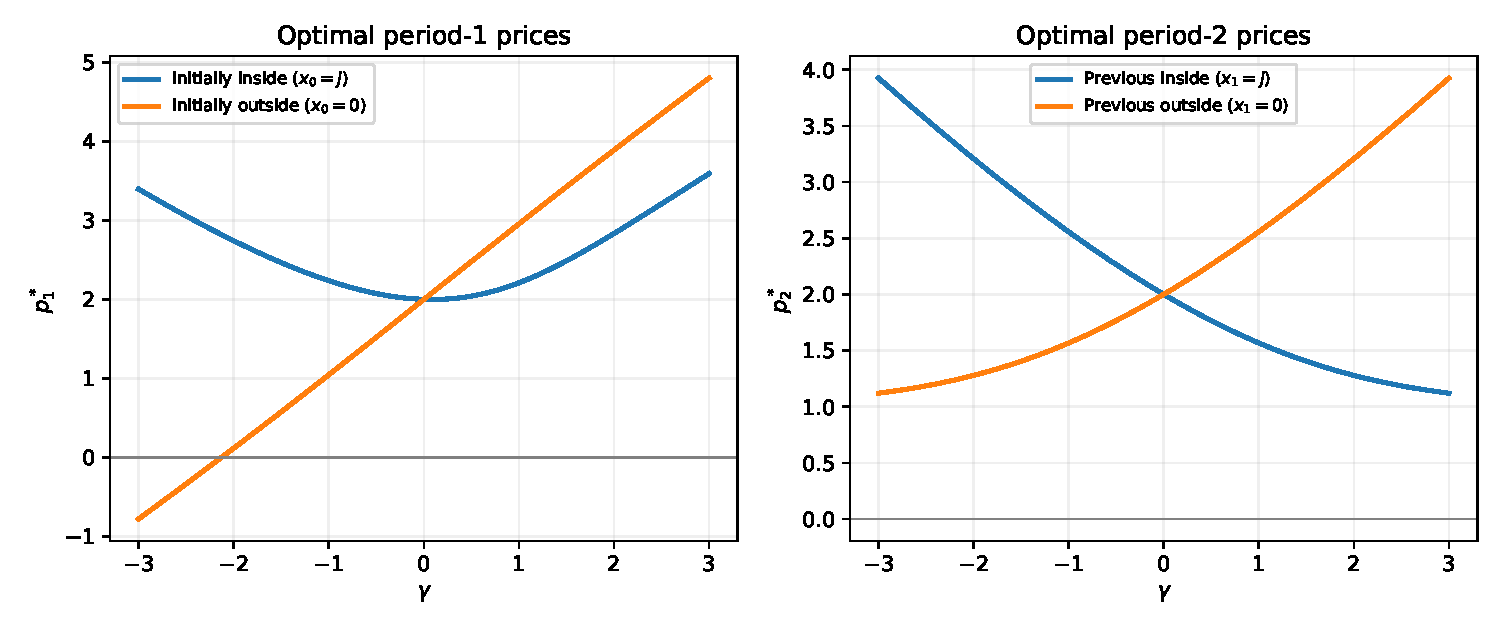
\includegraphics[width=\linewidth,height=.65\textheight,keepaspectratio]{assets/results/supply/optimal_prices_by_gamma.pdf}
\caption{Optimal prices by switching preference and initial state}
\label{fig:supply-prices}
\end{figure}
\FloatBarrier
\begin{figure}[htbp]
\centering
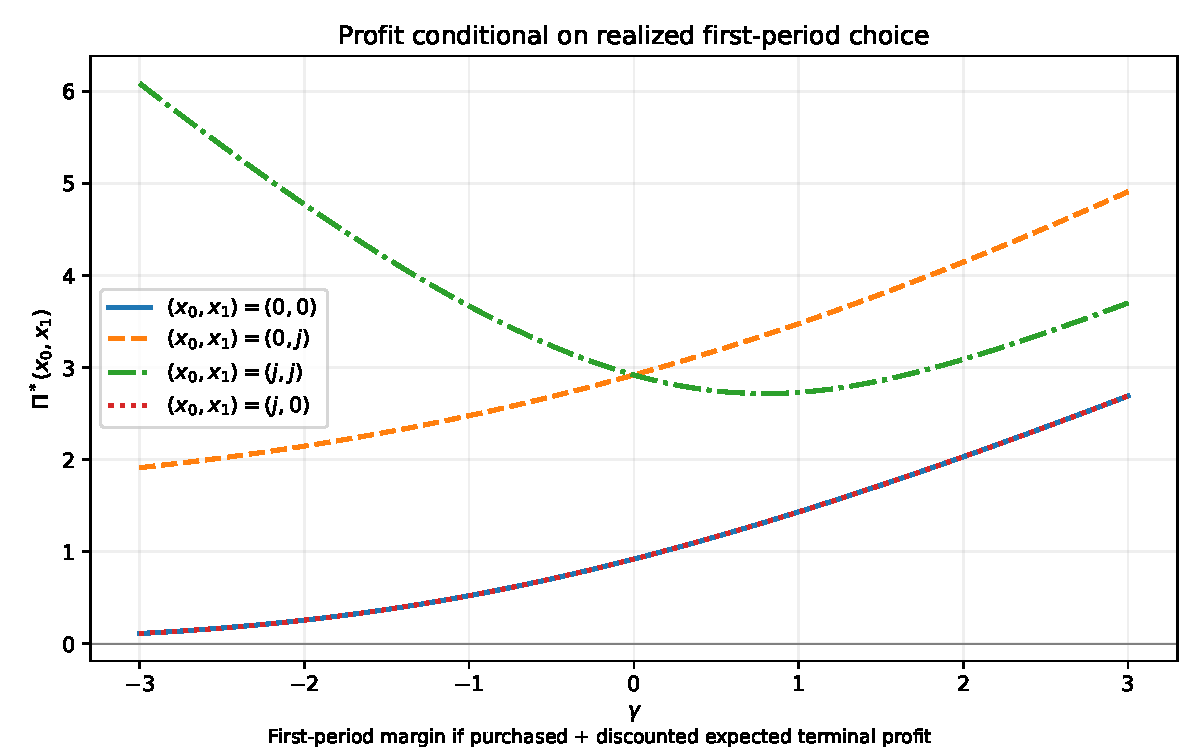
\includegraphics[width=\linewidth,height=.65\textheight,keepaspectratio]{assets/results/supply/all_state_realized_profit.pdf}
\caption{Profit conditional on initial state and first-period choice}
\label{fig:supply-history-profit}
\end{figure}
\FloatBarrier
\begin{figure}[htbp]
\centering
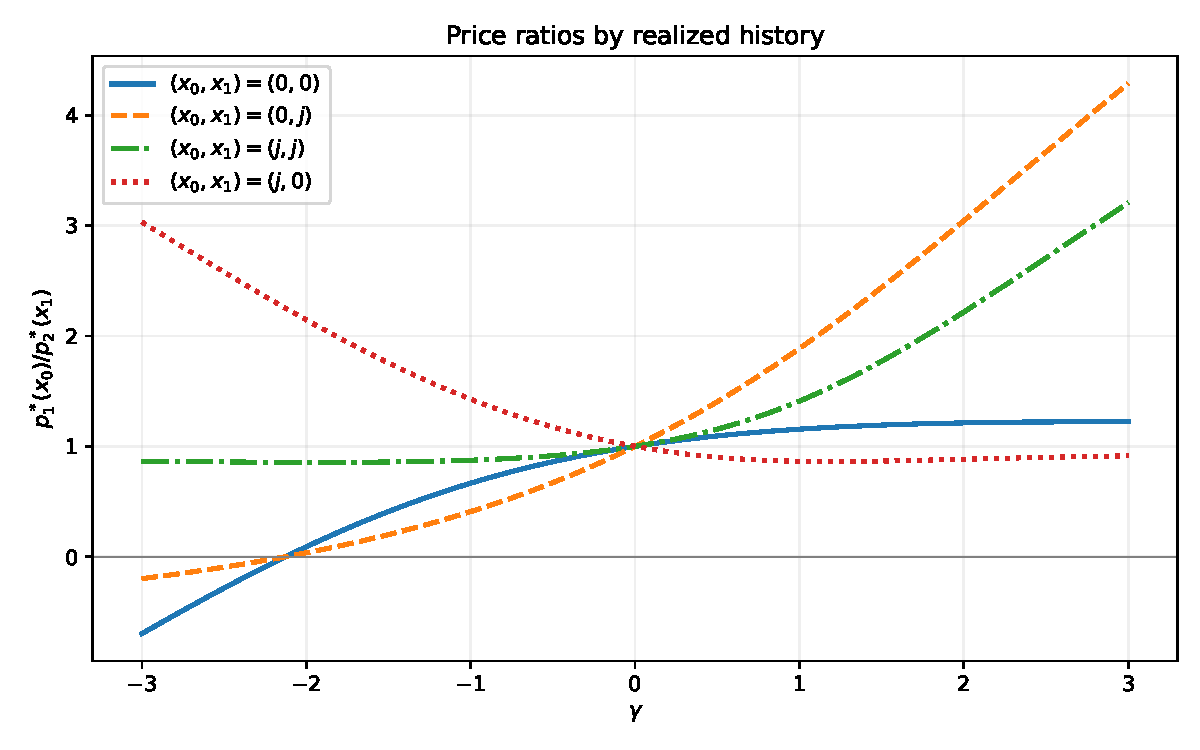
\includegraphics[width=\linewidth,height=.65\textheight,keepaspectratio]{assets/results/supply/all_state_price_ratios.pdf}
\caption{Price ratios conditional on consumption history}
\label{fig:supply-history-ratios}
\end{figure}
\FloatBarrier

\subsection{Uncertainty about Switching Type}
\label{subsec:gamma-uncertainty}
The initial purchase state $h$ is observed. The firm assigns fixed probabilities
to switching types:
\begin{equation}
 \gamma_r\in\{-1.25,0,1.25\},\qquad
 \lambda_r=\Pr(\gamma=\gamma_r),\qquad\sum_r\lambda_r=1.
\end{equation}
Compare the equal prior $(1/3,1/3,1/3)$ and the three permutations of
$(0.50,0.25,0.25)$. All other parameters retain the numerical supply calibration.
The firm keeps the same beliefs in both periods and after either purchase outcome:
\begin{equation}
 \lambda_{r,1}(h)=\lambda_{r,2}(j)=\lambda_{r,2}(0)=\lambda_r.
\end{equation}
History changes demand and terminal prices, but does not change type probabilities.
The fixed-belief mixture demand is
\begin{equation}
 A(p,h;\lambda)=\sum_r\lambda_r
 \frac{e^{\beta+\alpha p+q(h)\gamma_r}}
 {1+e^{\beta+\alpha p+q(h)\gamma_r}}.
\end{equation}
Terminal values and the first-period objective are
\begin{align}
 W(a;\lambda)&=\max_x A(x,a;\lambda)(x-c),\\
 \Pi^{\mathrm{fixed}}(h,\lambda)&=\max_p\bigl\{
 A(p,h;\lambda)(p-c)\notag\\
 &\quad+\delta[A(p,h;\lambda)W(j;\lambda)
 +(1-A(p,h;\lambda))W(0;\lambda)]\bigr\}.
\end{align}
The figures compare this fixed-belief objective with prior-weighted known-type
profit. The reported difference is
\begin{equation}
 \mathcal I(h,\lambda)=\sum_r\lambda_r\Pi_r^*(h)
 -\Pi^{\mathrm{fixed}}(h,\lambda).
\end{equation}
Derivations are in Appendix~\ref{app:gamma-uncertainty}.
\begin{table}[htbp]\centering\small
\caption{Pricing with known and uncertain switching types}
\label{tab:gamma-uncertainty}
\begin{tabular}{llrrr}\toprule
Initial state & Prior & Known profit & Uncertain profit & Information value\\\midrule
$j$ & Equal types & 2.2061 & 1.9460 & 0.2601 \\
$0$ & Equal types & 1.9799 & 1.9460 & 0.0339 \\
$j$ & Habit type more likely & 2.3843 & 2.1175 & 0.2668 \\
$0$ & Habit type more likely & 1.8312 & 1.7812 & 0.0499 \\
$j$ & Neutral type more likely & 2.1346 & 1.9337 & 0.2009 \\
$0$ & Neutral type more likely & 1.9649 & 1.9337 & 0.0312 \\
$j$ & Novelty type more likely & 2.0996 & 1.8368 & 0.2628 \\
$0$ & Novelty type more likely & 2.1437 & 2.1267 & 0.0169 \\
\bottomrule\end{tabular}
\end{table}

\FloatBarrier
\begin{figure}[htbp]
\centering
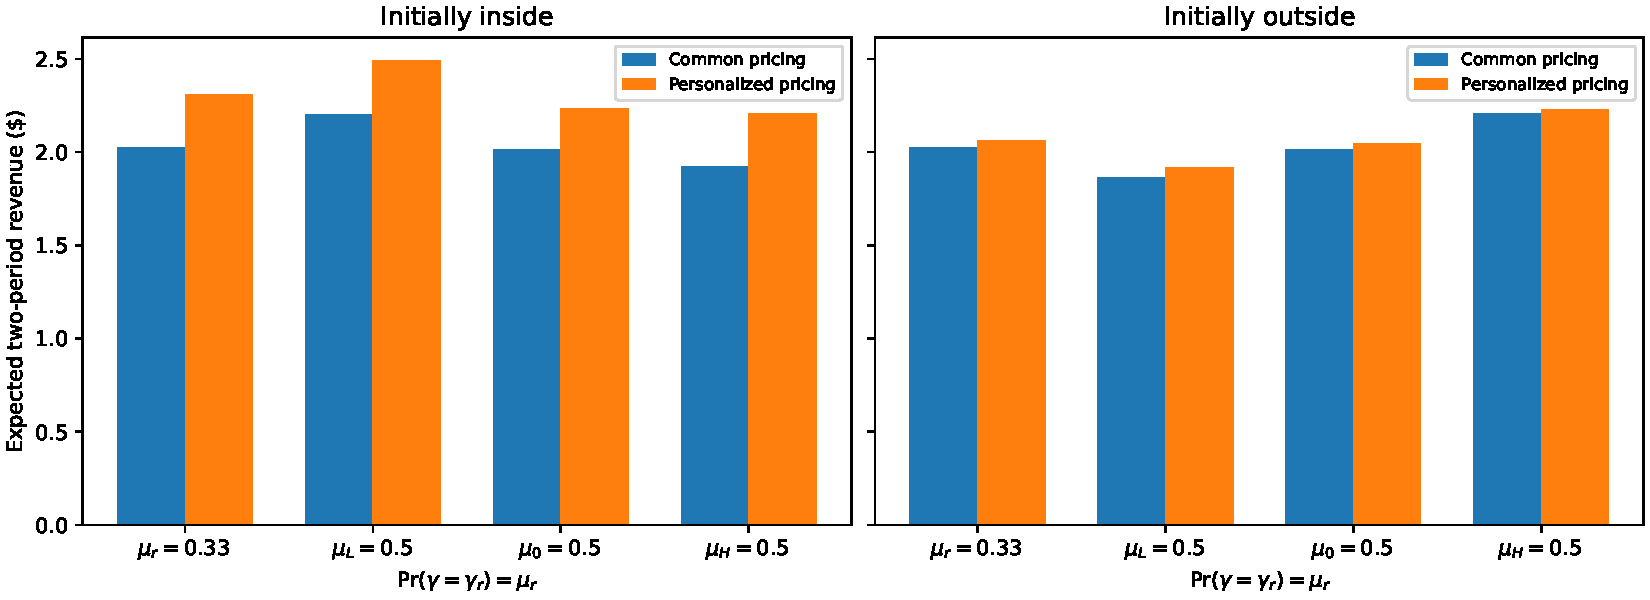
\includegraphics[width=\linewidth,height=.72\textheight,keepaspectratio]{assets/results/gamma_uncertainty/profits.pdf}
\caption{Optimized expected profit with known and uncertain switching types.}
\label{fig:gamma-profits}
\end{figure}
\FloatBarrier
\begin{figure}[htbp]
\centering
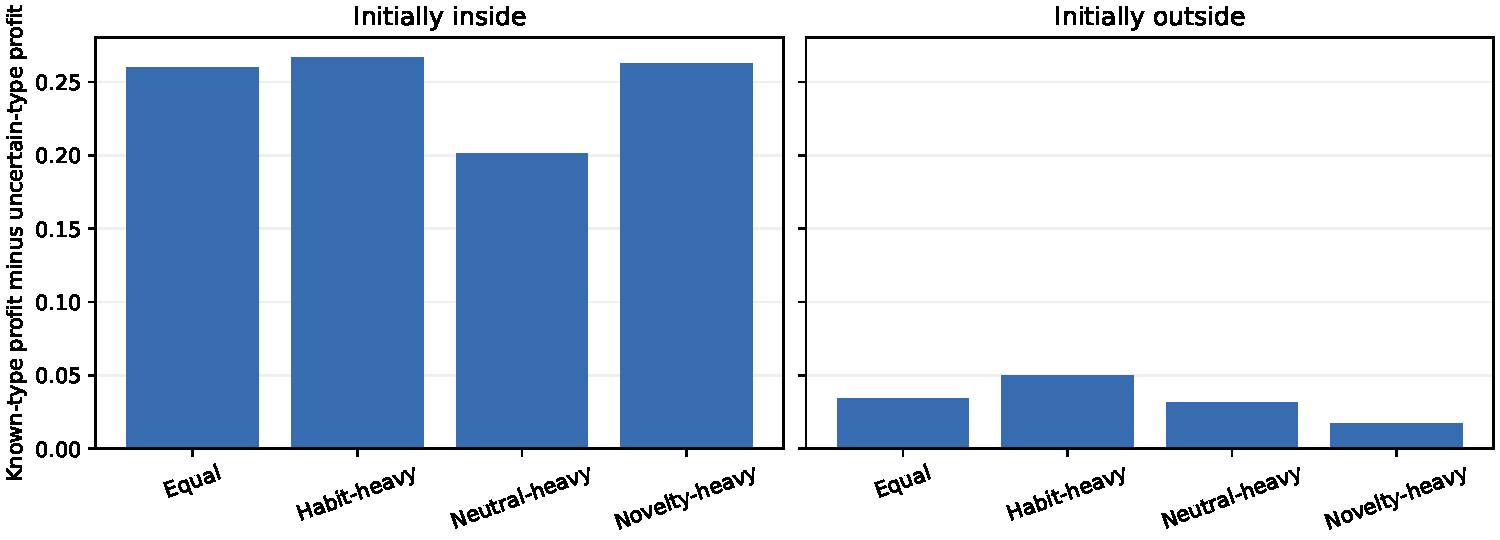
\includegraphics[width=\linewidth,height=.72\textheight,keepaspectratio]{assets/results/gamma_uncertainty/information_value.pdf}
\caption{Value of observing switching type, conditional on initial purchase state.}
\label{fig:gamma-information_value}
\end{figure}
\FloatBarrier

\section{Discussion of Theoretical Results}
\label{sec:theory-discussion}
% Author to write. Previous discussion is preserved in supply_previous.tex;
% its unconditional sign claims do not apply to the current model.

% ============================================================
% EMPIRICAL DEMAND SIDE
% ============================================================

\section{Data}
\label{sec:data}

\subsection{Data Sources}

\subsection{Sample Construction}

\subsection{Variable Construction}

\subsection{Summary Statistics}

% Aggregate sources: full_panel_overview.tex, matched_yogurt_overview.tex,
% full_panel_household_size.tex, and matched_yogurt_household_size.tex.
% Requires \usepackage{booktabs}.
\begin{table}[htbp]\centering\small
\centering
\caption{Summary statistics: full sample and yogurt sample}
\label{tab:full-panel-vs-yogurt}
\begin{adjustbox}{max width=\linewidth}
\begin{tabular}{lrr}
\toprule
 & Full sample & Yogurt sample \\
\midrule
\multicolumn{3}{l}{\textit{Sample and purchase activity}} \\
Households & 37,827 & 15,106 \\
Mean observed panel years & 3.96 & 3.16 \\
Mean trips per household & 493.13 & 20.26 \\
Mean trips per approximate observed week & 2.27 & 0.11 \\
Mean distinct UPCs per household & 1,178.31 & 13.89 \\
Mean purchase lines per household & 3,397.64 & 45.15 \\
Mean packages per household & 4,669.07 & 93.77 \\
Mean head age (category code) & 6.96 & 7.01 \\
Mean household income (category code) & 16.18 & 17.06 \\
Race: White (\%) & 80.33 & 81.58 \\
Race: Black (\%) & 12.81 & 12.15 \\
Race: Asian (\%) & 1.57 & 1.57 \\
Race: Other (\%) & 2.19 & 2.11 \\
Hispanic (\%) & 3.10 & 2.59 \\
\bottomrule
\end{tabular}
\end{adjustbox}
\end{table}

\FloatBarrier
\begin{table}[htbp]\centering\small
\caption{Matched yogurt sample: purchase dynamics}
\begin{adjustbox}{max width=\linewidth}
\begin{tabular}{lr}
\toprule
metric & value \\
\midrule
Matched households & 15106.00 \\
Observed yogurt purchase weeks & 282648.00 \\
Mean flavors bought per household & 10.76 \\
Mean household flavor HHI (0 to 1) & 0.32 \\
Mixed-flavor weeks (\%) & 37.88 \\
Weeks above seven packages (\%) & 21.72 \\
Eligible adjacent single-flavor week pairs & 30392.00 \\
Switch rate in eligible pairs (\%) & 46.75 \\
Mean single-flavor spell length (consecutive calendar weeks) & 1.10 \\
Median gap between purchase weeks & 3.00 \\
\bottomrule
\end{tabular}
\end{adjustbox}
\end{table}

\FloatBarrier
\begin{figure}[htbp]
\centering
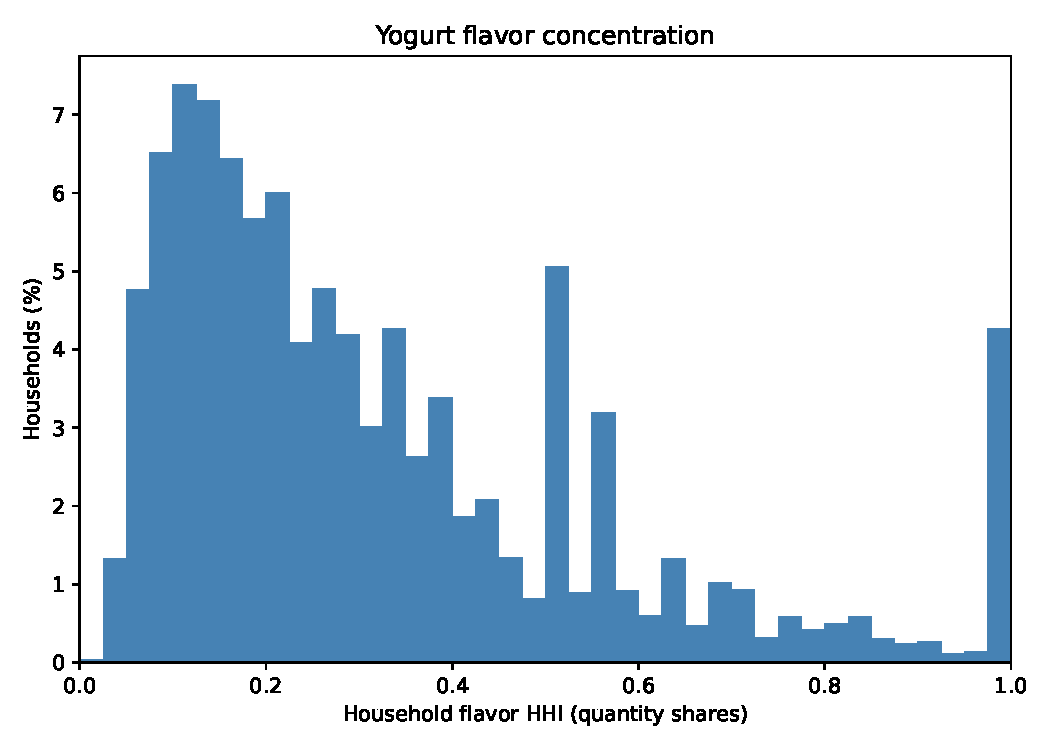
\includegraphics[width=\linewidth,height=.65\textheight,keepaspectratio]{assets/results/summary_statistics/flavor_hhi_histogram.pdf}
\caption{Distribution of household flavor concentration}
\label{fig:flavor-hhi}
\end{figure}
\FloatBarrier
\begin{figure}[htbp]
\centering
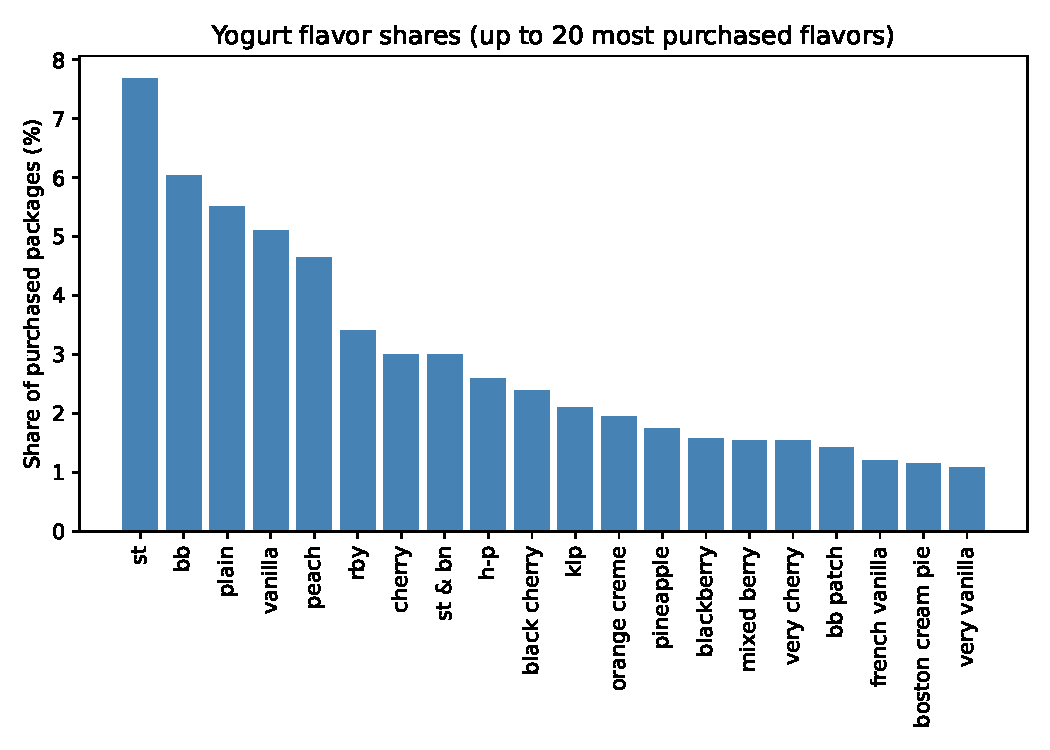
\includegraphics[width=\linewidth,height=.65\textheight,keepaspectratio]{assets/results/summary_statistics/flavor_shares.pdf}
\caption{Shares of purchased packages by detailed flavor}
\label{fig:flavor-shares}
\end{figure}
\FloatBarrier
\begin{figure}[htbp]
\centering
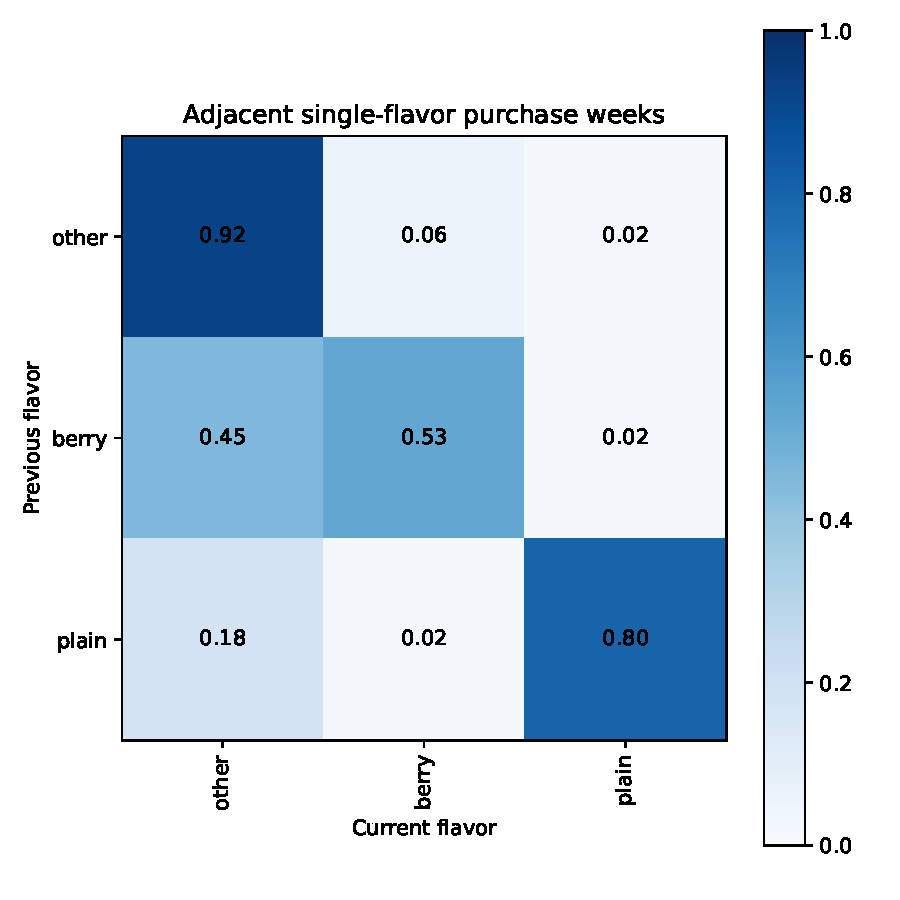
\includegraphics[width=\linewidth,height=.65\textheight,keepaspectratio]{assets/results/summary_statistics/aggregated_flavors/flavor_transitions.pdf}
\caption{Transitions across aggregated flavor groups}
\label{fig:flavor-transitions}
\end{figure}
\FloatBarrier

% ============================================================
% DEMAND MODEL
% ============================================================

\section{Demand Model}
\label{sec:demand-model}

\subsection{Choice Setting and Purchase History}
Let $i$ index consumers and $t$ calendar weeks. The inside alternatives are
\begin{equation*}
 \mathcal J=\{\mathrm{berry},\mathrm{plain},\mathrm{other}\}.
\end{equation*}
Alternative $0$ is the outside good. Let $y_{ijt}$ denote the number of packages
of flavor $j$ purchased in week $t$. For observed yogurt purchase weeks,
\begin{align}
 Q_{it}&=\sum_{j\in\mathcal J}y_{ijt},\\
 y_{i0t}&=\max\{0,7-Q_{it}\},\\
 M_{it}&=Q_{it}+y_{i0t}=\max\{7,Q_{it}\}.
\end{align}
Let $\mathcal H_i$ contain the observed purchase weeks used to construct history,
and $\mathcal T_i\subseteq\mathcal H_i$ the weeks retained for estimation.
The share of each inside flavor in a purchase week is
\begin{equation}
 w_{ijt}=\frac{y_{ijt}}{Q_{it}},\qquad t\in\mathcal H_i.
\end{equation}
Novelty is the share of other flavors purchased in the immediately preceding
calendar week:
\begin{equation}
 N_{ijt}=\begin{cases}
 \displaystyle\sum_{k\in\mathcal J,\,k\ne j}w_{ik,t-1}=1-w_{ij,t-1},
 &t-1\in\mathcal H_i,\\[3pt]
 0,&t-1\notin\mathcal H_i.
 \end{cases}
 \label{eq:empirical-novelty}
\end{equation}
Since $0\le w_{ij,t-1}\le1$, novelty satisfies $N_{ijt}\in[0,1]$.
It equals one when last week's basket contained other flavors and no $j$, and
zero when the basket contained only $j$.

For example, suppose last week a consumer bought three berry packages and one
plain package. The novelty of each possible flavor choice this week is
\begin{equation}
 \begin{aligned}
 N_{i,\mathrm{berry},t}&=1-\frac{3}{4}=0.25,\\
 N_{i,\mathrm{plain},t}&=1-\frac{1}{4}=0.75,\\
 N_{i,\mathrm{other},t}&=1-\frac{0}{4}=1.
 \end{aligned}
 \label{eq:novelty-example}
\end{equation}
Choosing berry differs from one quarter of last week's purchases; choosing
plain differs from three quarters; choosing other differs from all of them.
Thus $N_{ijt}$ measures switching intensity relative to the previous basket
for a possible choice of $j$, rather than the realized change in the entire
basket. Its contribution to utility is $\gamma_iN_{ijt}$: positive $\gamma_i$
rewards novelty, while negative $\gamma_i$ penalizes it.


The habit measure in the fitted model is cumulative own-flavor stock:
\begin{equation}
 H_{ijt}=\sum_{\substack{s\in\mathcal H_i\\s<t}}w_{ijs}.
 \label{eq:empirical-habit}
\end{equation}
Both histories start at zero. Missing purchase weeks contribute no stock and
set the next week's novelty measure to zero; they are not inserted as outside-choice weeks.

\subsection{Utility and Consumer Heterogeneity}
\begin{align}
 U_{ijt}&=V_{ijt}+\varepsilon_{ijt},\\
 V_{ijt}&=\beta_0+\beta_j+\gamma_iN_{ijt}+\phi_iH_{ijt}+\alpha_i p_{ijt},
 \qquad j\in\mathcal J,
 \label{eq:utility}\\
 U_{i0t}&=\varepsilon_{i0t},\qquad V_{i0t}=0.
\end{align}
The flavor constants are relative to other: $\beta_{\mathrm{other}}=0$.
The shocks are independent unit-scale Type-I extreme value.
The three random coefficients are fixed within consumer:
\begin{align}
 \alpha_i&=-\exp(\mu_\alpha+\sigma_\alpha\nu_{i\alpha}),\\
 \gamma_i&=\mu_\gamma+\sigma_\gamma\nu_{i\gamma},\\
 \phi_i&=\mu_\phi+\sigma_\phi\nu_{i\phi},\\
 \nu_i&=(\nu_{i\alpha},\nu_{i\gamma},\nu_{i\phi})'
 \sim\mathcal N(0,I_3).
\end{align}
Thus $\alpha_i<0$, while novelty and habit coefficients are unrestricted in sign.

\subsection{Choice Probabilities and Market Shares}
Let $\mathcal A_{it}\subseteq\mathcal J$ denote the flavors available at the
consumer's exposure store, and $\mathcal A_{it}^0=\mathcal A_{it}\cup\{0\}$.
Conditional on the consumer's type,
\begin{align}
 P_{ijt}(\nu_i;\theta)
 &=\frac{\exp\{V_{ijt}(\nu_i;\theta)\}}
 {1+\sum_{k\in\mathcal A_{it}}\exp\{V_{ikt}(\nu_i;\theta)\}},
 \qquad j\in\mathcal A_{it},
 \label{eq:choice-probability}\\
 P_{i0t}(\nu_i;\theta)
 &=\frac{1}{1+\sum_{k\in\mathcal A_{it}}\exp\{V_{ikt}(\nu_i;\theta)\}}.
\end{align}
Unavailable inside alternatives have zero probability.
Integrate over types before averaging across consumers:
\begin{align}
 \overline P_{ijt}(\theta)
 &=\int P_{ijt}(\nu;\theta)\varphi_3(\nu)\,d\nu,\\
 s_{jt}(\theta)&=\frac{1}{N_t}\sum_{i:\,t\in\mathcal T_i}\overline P_{ijt}(\theta).
\end{align}
Here $N_t$ is the number of retained consumers in week $t$.

\section{Estimation}
\label{sec:estimation}

\subsection{Identification}
\label{subsec:identification}
% Author to write: identifying variation, price exogeneity in the no-control
% specification, and conditioning on observed initial histories.

\subsection{Simulated Maximum Likelihood}
\label{subsec:estimation-procedure}
Conditional on a persistent consumer type, the panel likelihood is
\begin{equation}
 L_i(\nu;\theta)=\prod_{t\in\mathcal T_i}
 \prod_{j\in\mathcal A_{it}^0}P_{ijt}(\nu;\theta)^{y_{ijt}}.
\end{equation}
Integrating over types gives
\begin{equation}
 L_i(\theta)=\int L_i(\nu;\theta)\varphi_3(\nu)\,d\nu.
\end{equation}
Use $R=64$ standard normal draws per consumer, held fixed across weeks and
objective evaluations:
\begin{align}
 \widehat L_i(\theta)&=\frac{1}{64}\sum_{r=1}^{64}
 \prod_{t\in\mathcal T_i}\prod_{j\in\mathcal A_{it}^0}
 P_{ijt}(\nu_{ir};\theta)^{y_{ijt}},\\
 Q_{64}(\theta)&=-\sum_{i=1}^N\log\widehat L_i(\theta),
 \label{eq:estimation-objective}\\
 \widehat\theta&=\argmin_\theta Q_{64}(\theta).
\end{align}
Multinomial count constants do not depend on $\theta$ and are omitted.
Run three optimization starts and retain the solution with the lowest objective.
Appendix~\ref{app:estimation} gives the parameter vector, likelihood derivation,
and numerical evaluation.

\subsection{Inference}
% Author to write.

% ============================================================
% EMPIRICAL RESULTS
% ============================================================

\section{Results}
\label{sec:results}

\subsection{Demand Estimates}

\begin{table}[htbp]\centering\small
\caption{Demand estimates without price controls}
\label{tab:demand-estimates}
\begin{adjustbox}{max width=\linewidth}
\begin{tabular}{lrr}\toprule
Parameter & Estimate & Standard error\\\midrule
Inside constant $\beta_0$ & 1.2173 & 0.0035 \\
Berry vs. other & -0.6241 & 0.0034 \\
Plain vs. other & -0.2719 & 0.0054 \\
Mean price coefficient $E[\alpha_i]$ & -0.8940 & 0.0044 \\
Mean novelty & -0.7732 & 0.0095 \\
Mean habit & 0.0369 & 0.0002 \\
SD price coefficient $\mathrm{SD}(\alpha_i)$ & 0.9019 & 0.0099 \\
SD novelty & 0.8003 & 0.0085 \\
SD habit & 0.0783 & 0.0004 \\
\bottomrule\end{tabular}
\end{adjustbox}
\end{table}

\FloatBarrier

\subsection{Price Elasticities}

\subsection{State Dependence}

\subsection{Consumer Heterogeneity}

\begin{figure}[htbp]
\centering
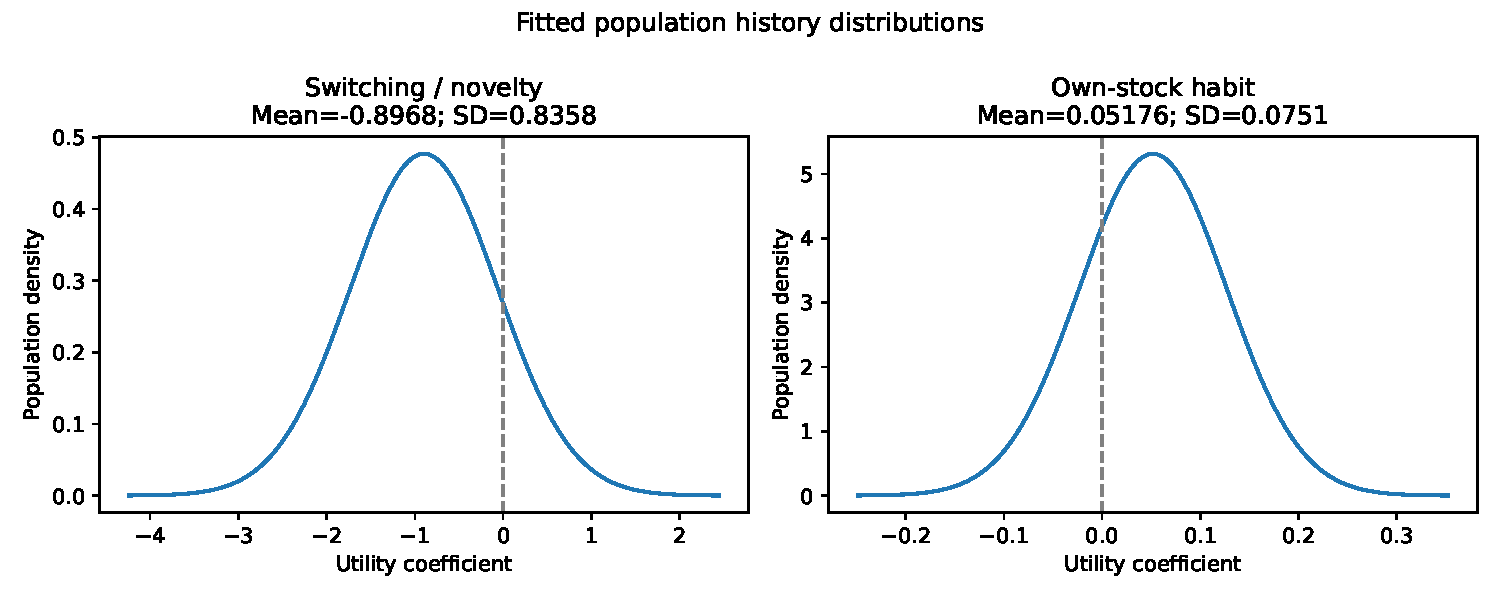
\includegraphics[width=\linewidth,height=.65\textheight,keepaspectratio]{assets/results/demand/history_distributions.pdf}
\caption{Estimated distributions of novelty and habit coefficients}
\label{fig:history-distributions}
\end{figure}
\FloatBarrier

% ============================================================
% ROBUSTNESS
% ============================================================
%
%\section{Robustness}
%\label{sec:robustness}
%
%\subsection{Alternative Specifications}
%
%\subsection{Alternative Samples}
%
%\subsection{Alternative Definitions}


% ============================================================
% DISCUSSION OF EMPIRICAL RESULTS
% ============================================================

\section{Discussion of Empirical Results}
\label{sec:empirical-discussion}

\subsection{Economic Magnitudes}

\begin{table}[htbp]\centering\small
\caption{Implied willingness to pay without price controls}
\label{tab:wtp-demand}
\begin{adjustbox}{max width=\linewidth}
\begin{tabular}{lrr}\toprule
Utility term & Mean WTP & Population SD\\\midrule
Inside constant $\beta_0$ & 2.7474 & 2.7716 \\
Berry vs. other & -1.4085 & 1.4210 \\
Plain vs. other & -0.6137 & 0.6192 \\
novelty & -1.7451 & 3.1116 \\
own stock & 0.0833 & 0.2647 \\
\bottomrule\end{tabular}
\end{adjustbox}
\end{table}

\FloatBarrier

\subsection{Relationship to Theoretical Predictions}

\subsection{Economic Interpretation}


% ============================================================
% SUPPLY-DEMAND CONNECTION
% ============================================================

\section{Connecting Demand Estimates to Firm Pricing}
\label{sec:supply-demand}

\subsection{Estimated Demand and Optimal Prices}

\subsubsection{Berry}
\begin{figure}[htbp]
\centering
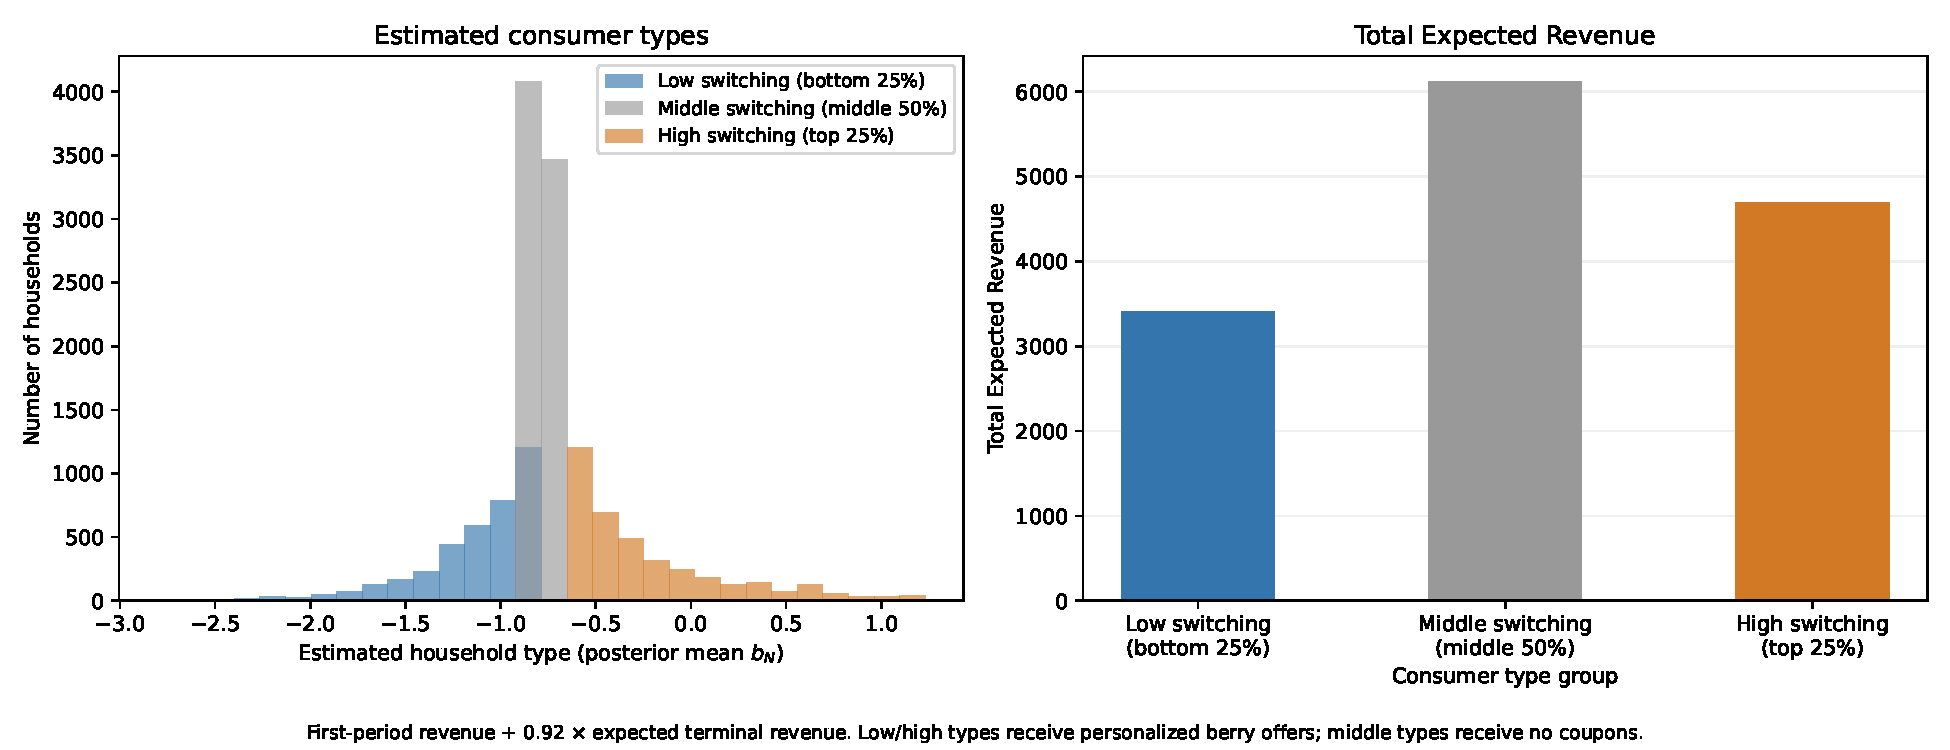
\includegraphics[width=\linewidth,height=.65\textheight,keepaspectratio]{assets/results/pricing/berry/household_coupon_results.pdf}
\caption{Berry: consumer types and expected revenue}
\label{fig:revenue-berry}
\end{figure}
\FloatBarrier
\begin{figure}[htbp]
\centering
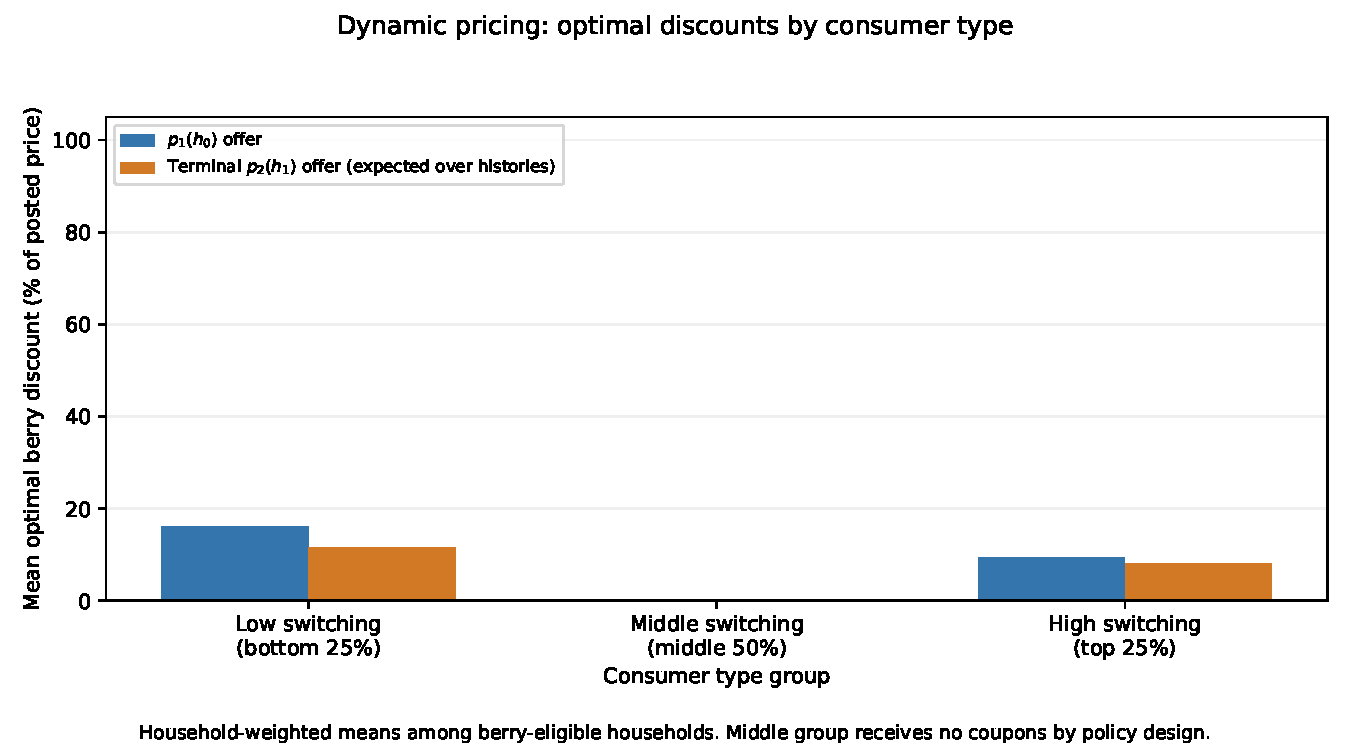
\includegraphics[width=\linewidth,height=.65\textheight,keepaspectratio]{assets/results/pricing/berry/discounts_by_consumer_type.pdf}
\caption{Berry: optimal offers by consumer type}
\label{fig:offers-berry}
\end{figure}
\FloatBarrier
\subsubsection{Plain}
\begin{figure}[htbp]
\centering
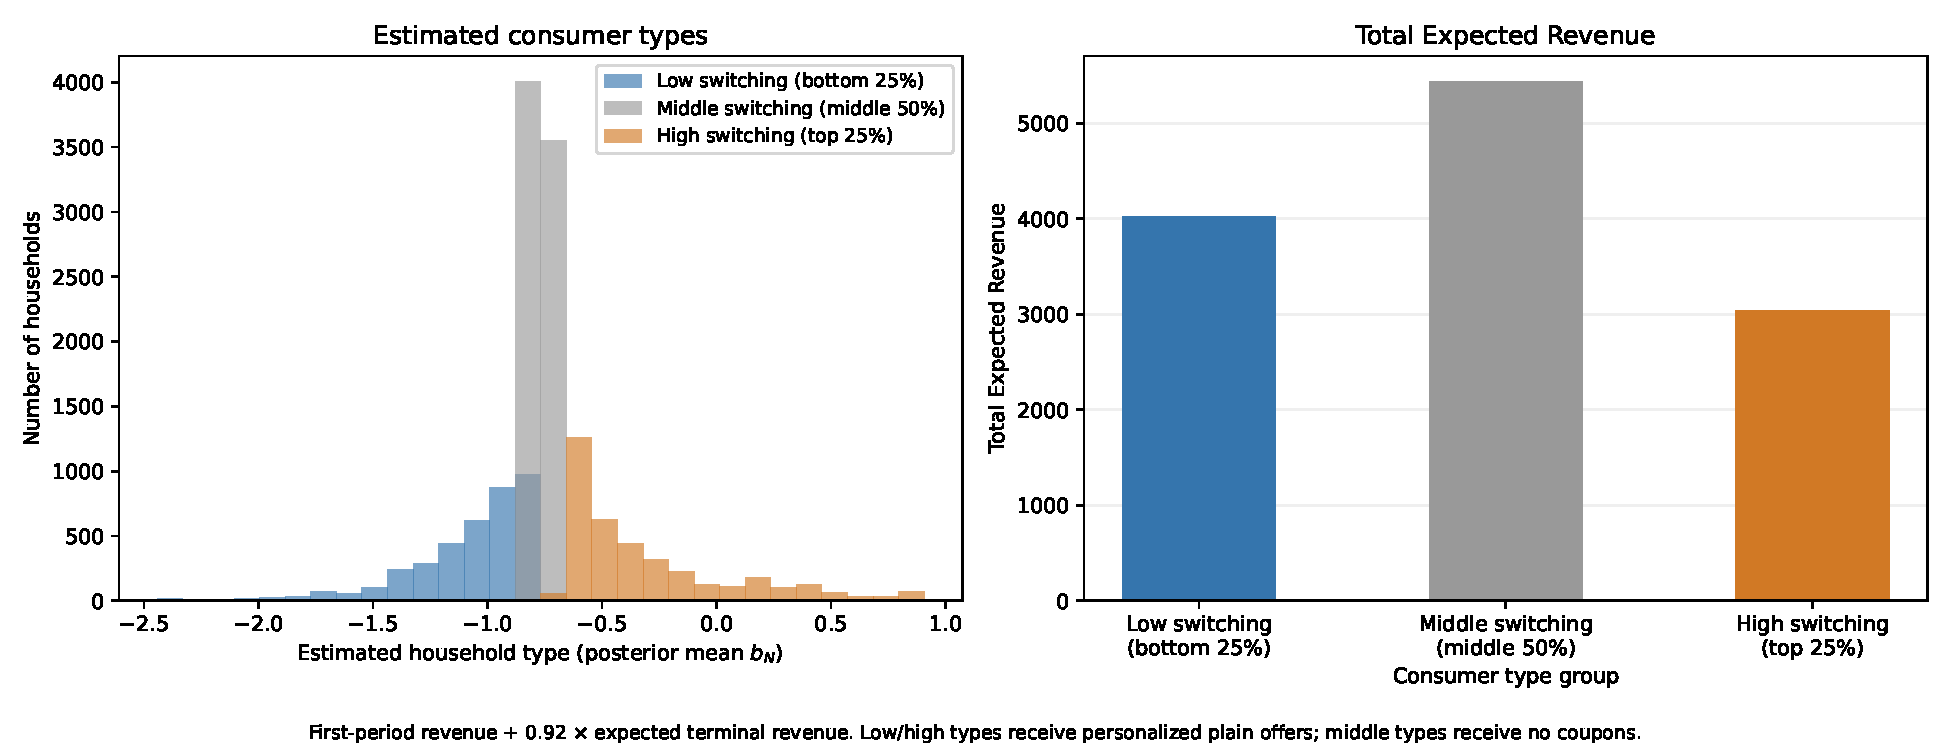
\includegraphics[width=\linewidth,height=.65\textheight,keepaspectratio]{assets/results/pricing/plain/household_coupon_results.pdf}
\caption{Plain: consumer types and expected revenue}
\label{fig:revenue-plain}
\end{figure}
\FloatBarrier
\begin{figure}[htbp]
\centering
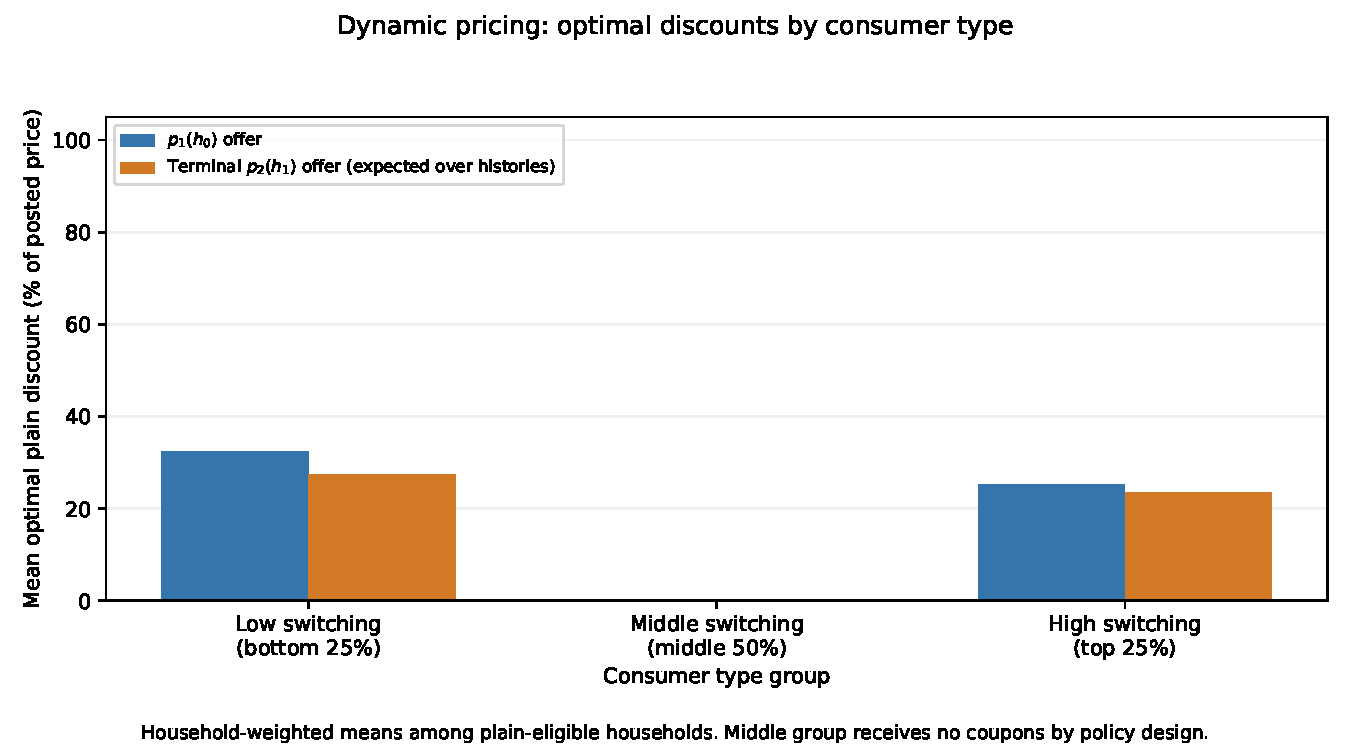
\includegraphics[width=\linewidth,height=.65\textheight,keepaspectratio]{assets/results/pricing/plain/discounts_by_consumer_type.pdf}
\caption{Plain: optimal offers by consumer type}
\label{fig:offers-plain}
\end{figure}
\FloatBarrier

\subsection{Counterfactual Pricing}

\begin{figure}[htbp]
\centering
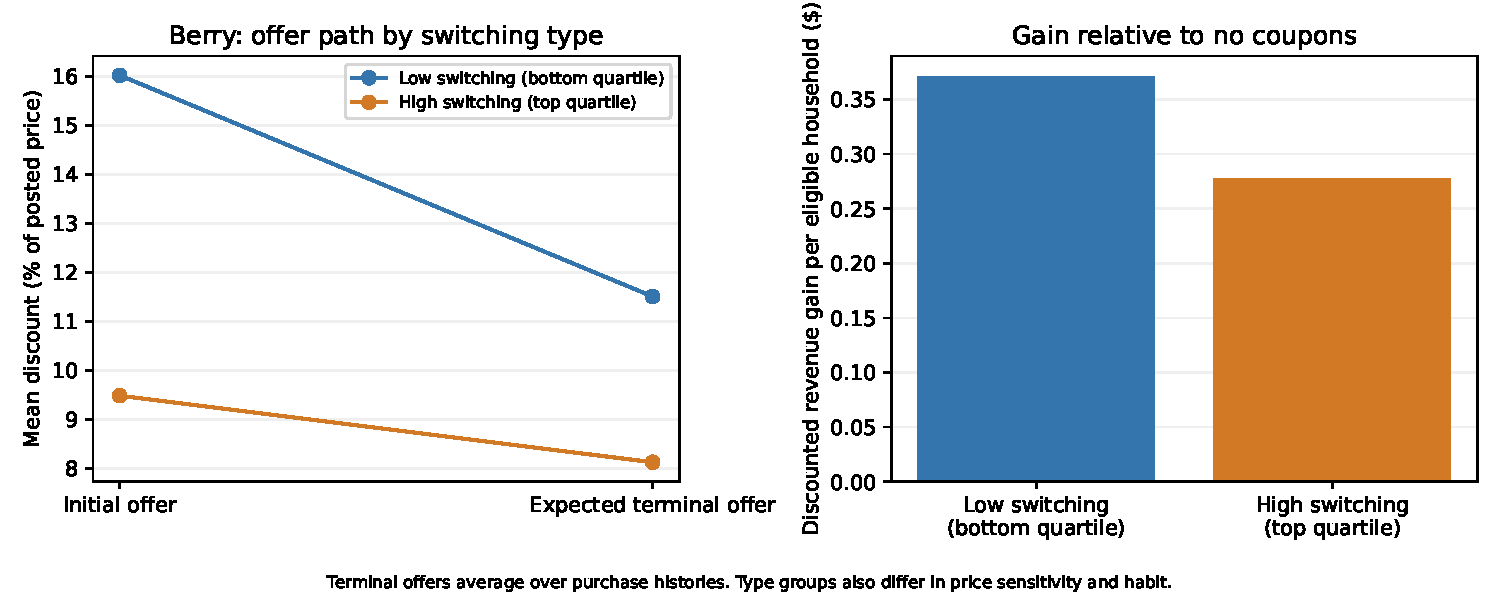
\includegraphics[width=\linewidth,height=.65\textheight,keepaspectratio]{assets/results/pricing/berry/pricing_mechanism.pdf}
\caption{Berry: initial offers and subsequent pricing}
\label{fig:mechanism-berry}
\end{figure}
\FloatBarrier
\begin{figure}[htbp]
\centering
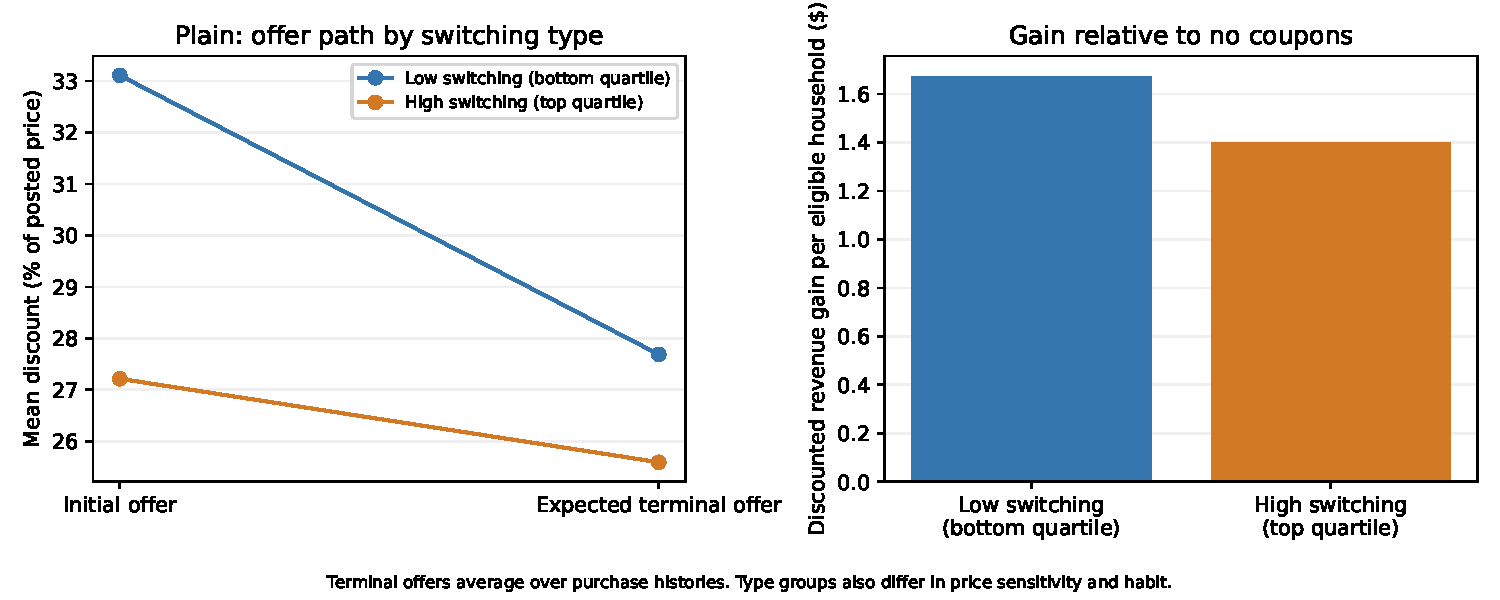
\includegraphics[width=\linewidth,height=.65\textheight,keepaspectratio]{assets/results/pricing/plain/pricing_mechanism.pdf}
\caption{Plain: initial offers and subsequent pricing}
\label{fig:mechanism-plain}
\end{figure}
\FloatBarrier

% Pending plots from the seminar presentation; enable once generated.
% \begin{figure}[htbp]
% \centering
% \includegraphics[width=\linewidth]{../../RESULTS_ONLY/pricing/plain/pricing_policy_benchmarks.pdf}
% \caption{Plain: pricing policy benchmarks}
% \end{figure}
% \begin{figure}[htbp]
% \centering
% \includegraphics[width=\linewidth]{../../RESULTS_ONLY/pricing/berry/pricing_policy_benchmarks.pdf}
% \caption{Berry: pricing policy benchmarks}
% \end{figure}
% \begin{figure}[htbp]
% \centering
% \includegraphics[width=\linewidth]{../../RESULTS_ONLY/pricing/plain/terminal_offers_by_purchase.pdf}
% \caption{Plain: terminal offers after purchase}
% \end{figure}

\subsection{Counterfactual Outcomes}

\begin{table}[htbp]\centering\small
\caption{Focal flavor comparison}
\label{tab:focal-flavor-comparison}
\begin{adjustbox}{max width=\linewidth}
\begin{tabular}{lrrrr}\toprule
 & \multicolumn{2}{c}{Plain} & \multicolumn{2}{c}{Berry}\\
 & No coupon & Personalized & No coupon & Personalized\\\midrule
Period 1 revenue & 5,910.49 & 6,593.19 & 6,873.53 & 7,296.20 \\
Period 2 revenue & 5,711.99 & 6,589.77 & 6,938.76 & 7,525.55 \\
Discounted revenue & 11,165.52 & 12,655.78 & 13,257.19 & 14,219.71 \\
Revenue change (\%) & 0.00 & 13.35 & 0.00 & 7.26 \\
Period 1 focal units & 3,088.87 & 4,004.99 & 7,521.02 & 8,283.57 \\
Period 2 focal units & 3,064.58 & 3,967.77 & 7,680.85 & 8,420.94 \\
Coupon expenditure & 0.00 & 4,014.12 & 0.00 & 2,842.89 \\
\bottomrule\end{tabular}
\end{adjustbox}
\end{table}

\FloatBarrier


% ============================================================
% COUNTERFACTUALS AND WELFARE
% ============================================================

\section{Counterfactuals and Welfare}
\label{sec:counterfactuals}

\subsection{Counterfactual Experiments}

\subsection{Consumer Surplus}

\subsection{Firm Profits}

\subsection{Total Welfare}


% ============================================================
% CONCLUSION
% ============================================================

\section{Conclusion}
\label{sec:conclusion}


% ============================================================
% REFERENCES
% ============================================================

\bibliographystyle{aer}
\bibliography{references}


% ============================================================
% APPENDIX
% ============================================================

\newpage
\appendix

\section{Supply-Side Derivations}
\label{app:supply}
\allowdisplaybreaks[1]

\subsection{Normalization and Demand Derivatives}
Subtracting outside deterministic utility gives
\begin{align}
 v_t(b)&=\beta+\alpha p_t(b)
 +\gamma\bigl[\mathbf{1}\{b=0\}-\mathbf{1}\{b=j\}\bigr]
 =\beta+\alpha p_t(b)+q(b)\gamma,\\
 \frac{\partial s_t}{\partial v_t}&=\frac{e^{v_t}}{(1+e^{v_t})^2}
 =s_t(1-s_t),\\
 ds_t&=s_t(1-s_t)[d\beta+p_t\,d\alpha+\alpha\,dp_t+q(b)\,d\gamma].
 \label{eq:supply-total-share}
\end{align}
The price and switching derivatives, holding history fixed, are
\begin{align}
 \frac{\partial s_t(h)}{\partial p_t(h)}&=\alpha s_t(h)s_{0t}(h),\\
 \left.\frac{\partial s_t(h)}{\partial\gamma}\right|_{p_t(h)}
 &=q(h)s_t(h)s_{0t}(h).
\end{align}
Multiplying the price derivatives by price and dividing by the corresponding
share gives the elasticities:
\begin{align}
 \epsilon_{jj,t}(h)&=\frac{p_t(h)}{s_t(h)}
 \frac{\partial s_t(h)}{\partial p_t(h)}
 =\alpha p_t(h)s_{0t}(h),\\
 \epsilon_{0j,t}(h)&=\frac{p_t(h)}{s_{0t}(h)}
 \frac{\partial s_{0t}(h)}{\partial p_t(h)}
 =-\alpha p_t(h)s_t(h).
\end{align}

\subsection{Backward Induction}
For either terminal state $a$,
\begin{align}
 \frac{d}{dp_2}\{s_2(p_2-c)\}
 &=s_2+\alpha s_2(1-s_2)(p_2-c)=0,\\
 1+\alpha(1-s_2^*)(p_2^*-c)&=0,\\
 p_2^*(a)-c&=-\frac{1}{\alpha[1-s_2^*(a)]},\\
 W_2(a)&=s_2^*(a)[p_2^*(a)-c]
 =-\frac{s_2^*(a)}{\alpha[1-s_2^*(a)]}.
\end{align}
Both continuation states enter first-period expected profit:
\begin{align}
 \Pi(p_1;h)&=s_1(p_1-c)+\delta[s_1W_2(j)+(1-s_1)W_2(0)]\\
 &=\delta W_2(0)+s_1[p_1-c+\delta\Delta W],\\
 \partial_{p_1}\Pi
 &=s_1+\alpha s_1(1-s_1)[p_1-c+\delta\Delta W],\\
 p_1^*-c+\delta\Delta W&=-\frac{1}{\alpha\ell},\\
 \Pi^*(h)&=\delta W_2(0)-\frac{s}{\alpha\ell}.
\end{align}

\subsection{Unique Global Optima}
Each pricing problem, up to an additive constant, has the form
\begin{equation}
 f(p)=s(p)(p-k),\quad s(p)=\frac{e^{b+\alpha p}}{1+e^{b+\alpha p}},
 \quad k=c\ \text{or}\ k=c-\delta\Delta W.
\end{equation}
\begin{align}
 f'(p)&=\frac{s(p)}{1+e^{b+\alpha p}}H(p),\\
 H(p)&=1+e^{b+\alpha p}+\alpha(p-k),\\
 H'(p)&=\alpha[1+e^{b+\alpha p}]<0,\\
 \lim_{p\to-\infty}H(p)&=+\infty,\qquad
 \lim_{p\to+\infty}H(p)=-\infty.
\end{align}
Thus $f'$ changes from positive to negative at a unique finite price,
which is the global maximizer. The first-period optimum can be below $c$.

\subsection{General Implicit and Envelope Derivatives}
For $\theta\in\{\gamma,\beta,\alpha,\delta\}$, define direct utility responses
\begin{align}
 D_{1\theta}&=\mathbf{1}\{\theta=\beta\}
 +p_1^*\mathbf{1}\{\theta=\alpha\}+q(h)\mathbf{1}\{\theta=\gamma\},\\
 D_{2\theta}(a)&=\mathbf{1}\{\theta=\beta\}
 +p_2^*(a)\mathbf{1}\{\theta=\alpha\}+q(a)\mathbf{1}\{\theta=\gamma\}.
\end{align}
The terminal envelope theorem and first-order condition imply
\begin{align}
 W_{2,\theta}(a)
 &=s_2^*(a)[1-s_2^*(a)]D_{2\theta}(a)[p_2^*(a)-c]
 =-\frac{s_2^*(a)D_{2\theta}(a)}{\alpha},\\
 0&=\frac{dp_2^*(a)}{d\theta}
 -\frac{\mathbf{1}\{\theta=\alpha\}}{\alpha^2[1-s_2^*(a)]}
 +\frac{ds_2^*(a)/d\theta}{\alpha[1-s_2^*(a)]^2},\\
 \frac{ds_2^*(a)}{d\theta}
 &=s_2^*(a)[1-s_2^*(a)]\left[D_{2\theta}(a)
 +\alpha\frac{dp_2^*(a)}{d\theta}\right],\\
 \frac{dp_2^*(a)}{d\theta}
 &=\frac{\mathbf{1}\{\theta=\alpha\}}{\alpha^2}
 -\frac{s_2^*(a)D_{2\theta}(a)}{\alpha}.
\end{align}
For the first-period pricing equation,
\begin{align}
 F&=p_1-c+\frac{1}{\alpha(1-s_1)}+\delta\Delta W=0,\\
 F_{p_1}&=1+\frac{s}{\ell}=\frac{1}{\ell},\\
 F_\theta&=-\frac{\mathbf{1}\{\theta=\alpha\}}{\alpha^2\ell}
 +\frac{sD_{1\theta}}{\alpha\ell}
 +\mathbf{1}\{\theta=\delta\}\Delta W+\delta\Delta W_\theta,\\
 \frac{dp_1^*}{d\theta}&=-\frac{F_\theta}{F_{p_1}}
 =\frac{\mathbf{1}\{\theta=\alpha\}}{\alpha^2}
 -\frac{sD_{1\theta}}{\alpha}
 -\ell[\mathbf{1}\{\theta=\delta\}\Delta W+\delta\Delta W_\theta].
 \label{eq:supply-general-derivative}
\end{align}
The continuation-value differences needed here are
\begin{align}
 \Delta W_\gamma&=(u+v)/\alpha,\\
 \Delta W_\beta&=(v-u)/\alpha,\\
 \Delta W_\alpha&=[vp_2^*(0)-up_2^*(j)]/\alpha,\\
 \Delta W_\delta&=0.
\end{align}
Substitution into \eqref{eq:supply-general-derivative} gives all four
first-period comparative statics in the text. In particular,
\begin{equation}
 W_2(j)\big|_{\gamma=0}=W_2(0)\big|_{\gamma=0},\qquad
 \Delta W_\gamma=B/\alpha<0
 \ \Longrightarrow\ \operatorname{sgn}(\Delta W)=-\operatorname{sgn}(\gamma).
\end{equation}
Together with $dp_1^*/d\delta=-\ell\Delta W$, this gives the discount-factor sign.

\subsection{Switching Derivatives and Conditional Signs}
Write a prime for a total derivative with respect to $\gamma$.
\begin{align}
 p_2^{*\prime}(a)&=-q(a)s_2^*(a)/\alpha,\\
 W_2'(a)&=-q(a)s_2^*(a)/\alpha,\\
 p_1^{*\prime}(h)&=-[q(h)s+\delta\ell B]/\alpha,\\
 s'&=s\ell[q(h)+\alpha p_1^{*\prime}]
 =s\ell^2[q(h)-\delta B],\\
 u'&=-u(1-u)^2,\\
 v'&=v(1-v)^2.
\end{align}
Applying the first-period envelope theorem retains both branches:
\begin{align}
 \Pi^{*\prime}(h)
 &=q(h)s\ell[p_1^*-c+\delta\Delta W]
 +\delta[sW_2'(j)+\ell W_2'(0)]\\
 &=-\frac{q(h)s}{\alpha}
 +\frac{\delta}{\alpha}[su-\ell v].
\end{align}
For $h=0$, the numerators in the price and profit expressions give
\begin{equation}
 p_1^{*\prime}(0)=-\frac{s+\delta\ell B}{\alpha}>0,\qquad
 \Pi^{*\prime}(0)=-\frac{s(1-\delta u)+\delta\ell v}{\alpha}>0,
\end{equation}
since $\delta u<1$. For $h=j$,
\begin{equation}
 p_1^{*\prime}(j)=\frac{s-\delta\ell B}{\alpha},\qquad
 \Pi^{*\prime}(j)=\frac{s(1+\delta u)-\delta\ell v}{\alpha}.
\end{equation}
Division by $\alpha<0$ gives the conditional inequalities in the text;
equality gives a zero derivative and reversing each inequality gives a negative derivative.

\subsection{Higher Derivatives and Ratios}
Using $\ell'=-s'$ and $B'=u'+v'$,
\begin{align}
 p_1^{*\prime\prime}
 &=-\frac{[q(h)-\delta B]s'+\delta\ell B'}{\alpha}
 =-\frac{s\ell^2[q(h)-\delta B]^2+\delta\ell B'}{\alpha},\\
 \frac{d^2p_1^*}{d\gamma\,d\beta}
 &=\frac{-s'+\delta[\ell(u'-v')-s'(u-v)]}{\alpha}.
\end{align}
For each fixed pair $(h,a)$, the quotient rule gives
\begin{align}
 R_{h,a}'&=\frac{p_2^*(a)p_1^{*\prime}(h)-p_1^*(h)p_2^{*\prime}(a)}{[p_2^*(a)]^2}\\
 &=\frac{-p_2^*(a)[q(h)s+\delta\ell B]
 +p_1^*(h)q(a)s_2^*(a)}{\alpha[p_2^*(a)]^2}.
\end{align}
No common sign follows across histories. The ratios require nonzero terminal
prices. When $c\ge0$, \eqref{eq:supply-terminal} gives $p_2^*(a)>0$.

\subsection{Profit Conditional on the First-Period Realization}
\begin{align}
 \Pi^*(h,j)&=p_1^*(h)-c+\delta W_2(j),\\
 \Pi^*(h,0)&=\delta W_2(0),\\
 s\Pi^*(h,j)+\ell\Pi^*(h,0)
 &=s[p_1^*(h)-c]+\delta[sW_2(j)+\ell W_2(0)]
 =\Pi^*(h).
\end{align}
Terminal profit remains expected conditional on $a$; fully realized profit also
conditions on the second-period choice.

\subsection{Uncertain Switching Type: Fixed Beliefs}
\label{app:gamma-uncertainty}
For each history $a$, the same fixed probabilities enter mixture demand:
\begin{align}
 A(x,a;\lambda)&=\sum_r\lambda_rs_r(x,a),\\
 A_x(x,a;\lambda)&=\sum_r\lambda_r\alpha s_r(x,a)[1-s_r(x,a)].
\end{align}
Terminal pricing solves
\begin{align}
 W(a;\lambda)&=\max_x A(x,a;\lambda)(x-c),\\
 0&=A(x,a;\lambda)+(x-c)A_x(x,a;\lambda).
\end{align}
Let $\Delta W(\lambda)=W(j;\lambda)-W(0;\lambda)$. Since beliefs are fixed,
these continuation values do not depend on the first-period price:
\begin{align}
 \Pi(p;h,\lambda)
 &=\delta W(0;\lambda)
 +A(p,h;\lambda)[p-c+\delta\Delta W(\lambda)],\\
 0&=A(p,h;\lambda)
 +A_p(p,h;\lambda)[p-c+\delta\Delta W(\lambda)],\\
 p_1^*(h;\lambda)
 &=c-\delta\Delta W(\lambda)
 -\frac{A(p_1^*,h;\lambda)}{A_p(p_1^*,h;\lambda)}.
\end{align}
Unlike a single-type logit, the mixture generally has no single-share logit
markup formula. Numerical optimization searches the mixture objective directly.
The belief vector is unchanged after either outcome. This is a fixed-belief
approximation: continuation demand is evaluated using $\lambda$, rather than the
Bayesian type composition of consumers reaching each state. Reported uncertain-type
profits are evaluated under that same fixed-belief objective.

The solver compares all grid-detected local maxima and repeats the first-price
search on a wider grid. Independent terminal maximizations and finite differences
check the solution. Degenerate type probabilities reproduce the known-type
solution; both terminal states retain exactly the original probability vector.
\begin{figure}[htbp]
\centering
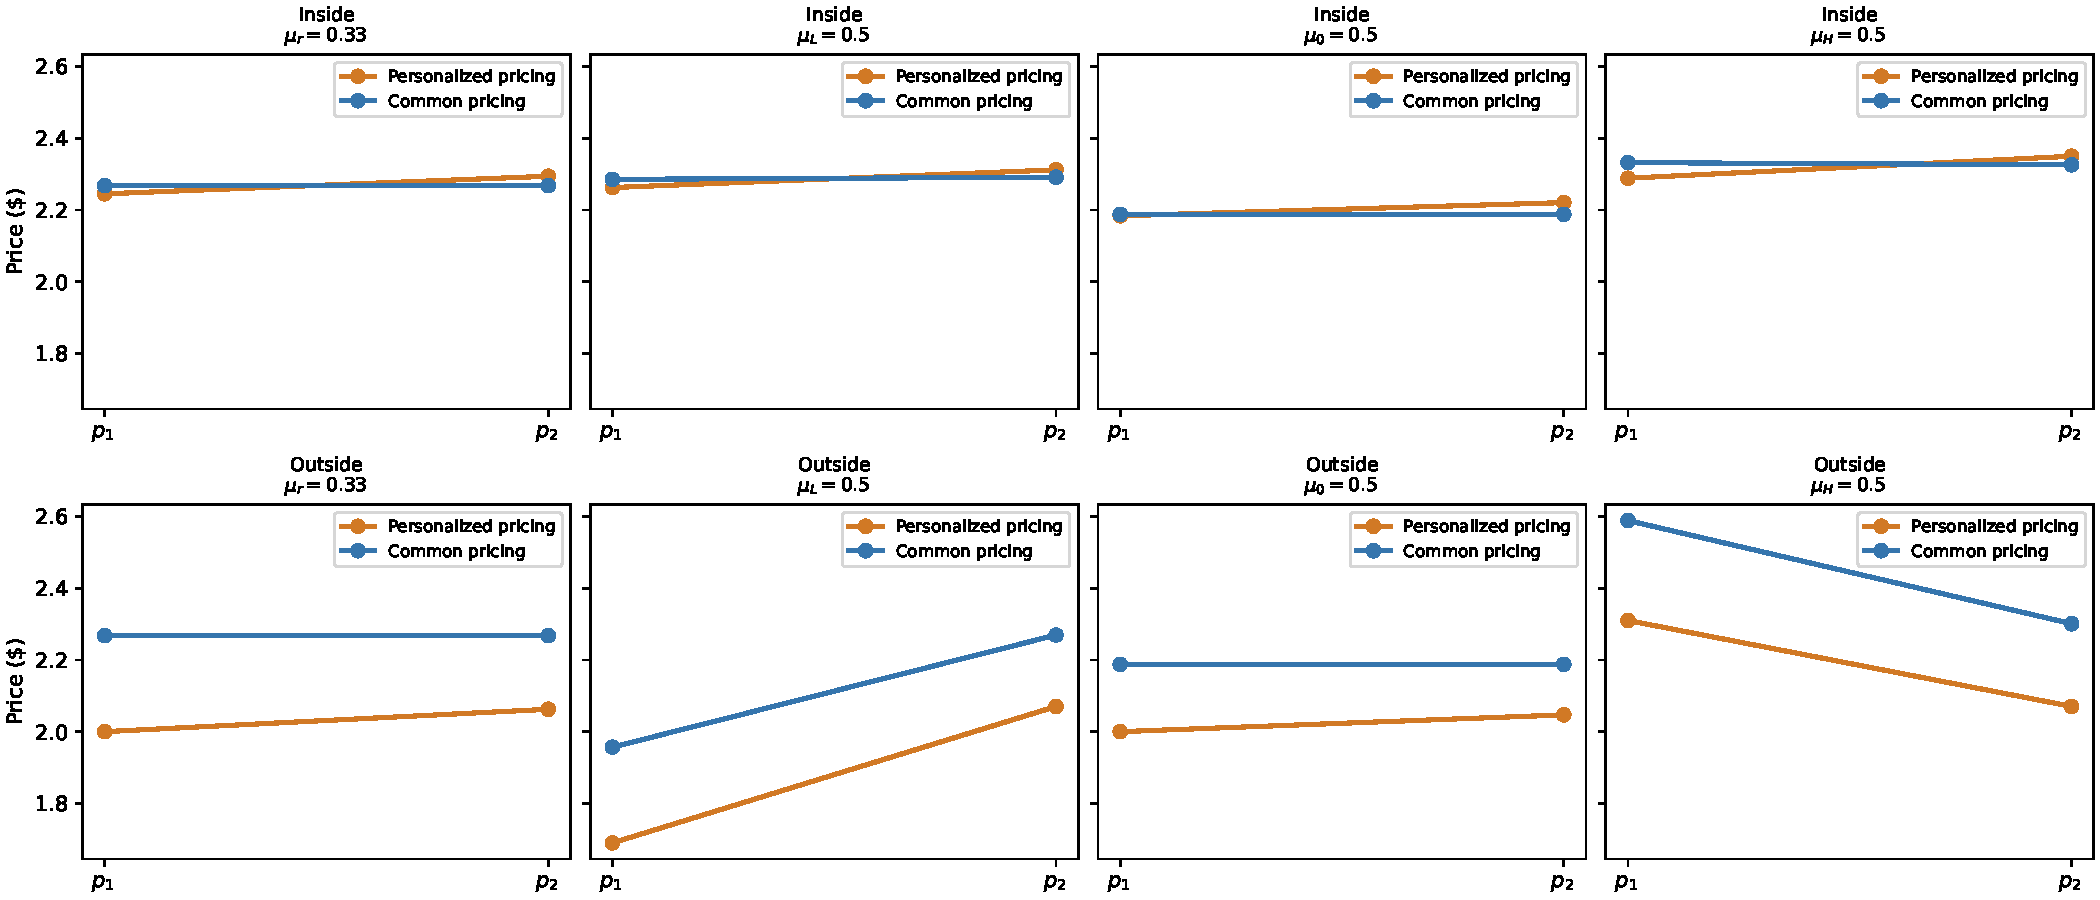
\includegraphics[width=\linewidth,height=.72\textheight,keepaspectratio]{assets/results/gamma_uncertainty/first_prices.pdf}
\caption{Expected first-period offered prices. Known-type prices are averaged using the prior.}
\label{fig:gamma-first_prices}
\end{figure}
\FloatBarrier
\begin{figure}[htbp]
\centering
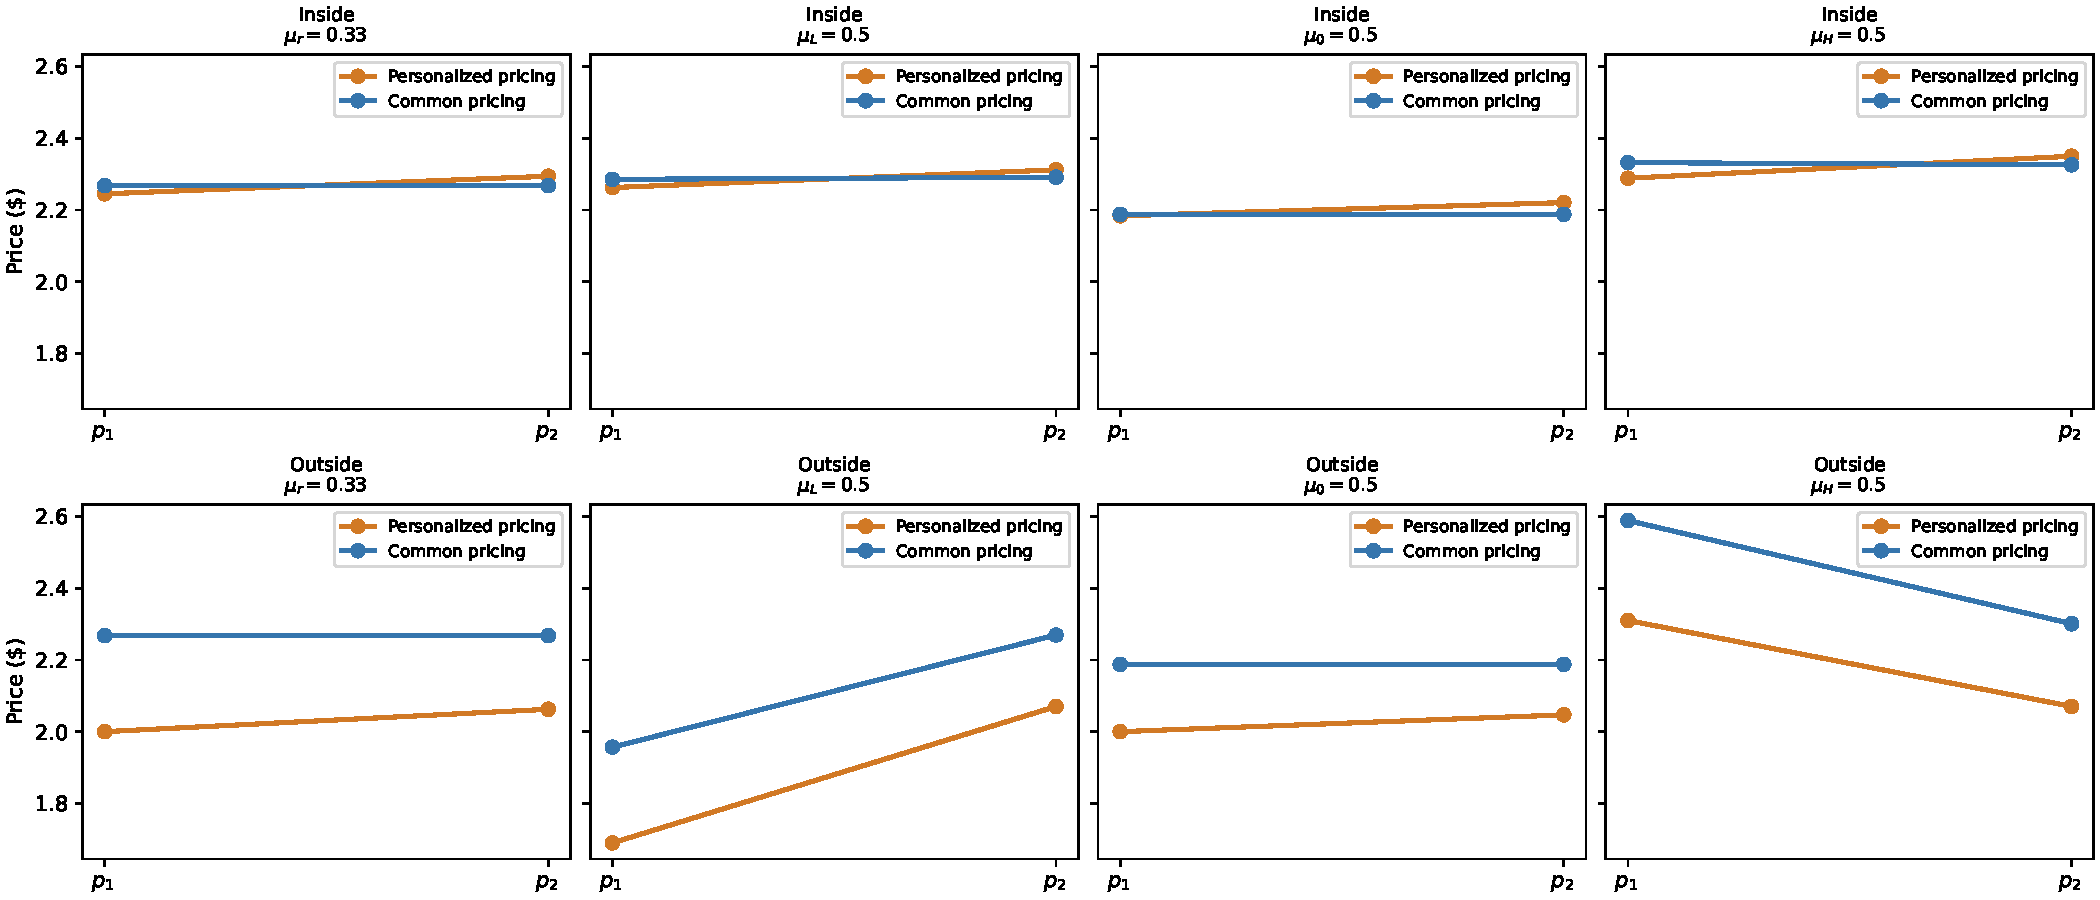
\includegraphics[width=\linewidth,height=.72\textheight,keepaspectratio]{assets/results/gamma_uncertainty/terminal_prices.pdf}
\caption{Expected terminal offered prices, averaging over type and first-period purchase outcomes.}
\label{fig:gamma-terminal_prices}
\end{figure}
\FloatBarrier

\section{Additional Data Details}
\label{app:data}


\section{Empirical Demand and Estimation Derivations}
\label{app:estimation}

\subsection{Parameters and Purchase Histories}
The estimated parameter vector is
\begin{equation}
 \theta=(\beta_0,\beta_{\mathrm{berry}},\beta_{\mathrm{plain}},
 \mu_\alpha,\sigma_\alpha,\mu_\gamma,\sigma_\gamma,\mu_\phi,\sigma_\phi)'.
\end{equation}
The main-text history measures correspond to the separate-history specification
in the estimator. For an adjacent prior purchase week,
\begin{align}
 N_{ijt}&=\sum_{k\ne j}w_{ik,t-1}\\
 &=\frac{\sum_{k\ne j}y_{ik,t-1}}{Q_{i,t-1}}
 =1-\frac{y_{ij,t-1}}{Q_{i,t-1}}.
\end{align}
If the prior basket contains only flavor $k$, then
\begin{equation}
 N_{ijt}=\mathbf{1}\{k\ne j\}.
\end{equation}
The share measure therefore reduces to the slides' switching indicator for
single-flavor baskets, while retaining mixed-flavor observations.
Equation~\eqref{eq:novelty-example} illustrates the calculation for a mixed basket.
The stock $H_{ijt}$ sums weekly own-flavor shares without depreciation or
normalization by the number of previous weeks. Each observed purchase week adds
one unit across flavors:
\begin{equation}
 \sum_{j\in\mathcal J}H_{ijt}
 =\#\{s\in\mathcal H_i:s<t\}.
\end{equation}
Histories are constructed before likelihood exclusions. Current purchases update
the stock only after the current week's predictors are recorded.

\subsection{Logit Probabilities}
For $j\in\mathcal A_{it}^0$, the probability that utility from $j$ exceeds utility
from all other alternatives is
\begin{align}
 P_{ijt}(\nu;\theta)
 &=\Pr\!\left(\varepsilon_{ikt}-\varepsilon_{ijt}
 \le V_{ijt}-V_{ikt}\ \text{for all }k\ne j\mid\nu\right)\\
 &=\int_{-\infty}^{\infty} f(e)
 \prod_{k\ne j}F(e+V_{ijt}-V_{ikt})\,de.
\end{align}
For Type-I extreme-value shocks,
\begin{equation}
 F(e)=\exp(-e^{-e}),\qquad f(e)=e^{-e}\exp(-e^{-e}).
\end{equation}
Writing $A=\sum_{k\in\mathcal A_{it}^0}\exp(V_{ikt}-V_{ijt})$ and using $z=e^{-e}$,
\begin{align}
 P_{ijt}(\nu;\theta)
 &=\int_{-\infty}^{\infty}e^{-e}\exp(-Ae^{-e})\,de\\
 &=\int_0^\infty e^{-Az}\,dz
 =\frac{1}{A}\\
 &=\frac{\exp(V_{ijt})}{\sum_{k\in\mathcal A_{it}^0}\exp(V_{ikt})}.
\end{align}
Setting $V_{i0t}=0$ gives the denominators in the main text.

\subsection{Weekly Counts and the Panel Likelihood}
Conditional on type and the observed pre-choice history, the multinomial
probability of a weekly count vector is
\begin{equation}
 f(y_{it}\mid\nu;\theta)
 =\frac{M_{it}!}{\prod_{j\in\mathcal A_{it}^0}y_{ijt}!}
 \prod_{j\in\mathcal A_{it}^0}P_{ijt}(\nu;\theta)^{y_{ijt}}.
\end{equation}
The product of factorial terms is independent of $\theta$. Dropping this factor,
\begin{align}
 L_i(\nu;\theta)
 &=\prod_{t\in\mathcal T_i}\prod_{j\in\mathcal A_{it}^0}
 P_{ijt}(\nu;\theta)^{y_{ijt}},\\
 \ell_i(\nu;\theta)
 &=\sum_{t\in\mathcal T_i}\sum_{j\in\mathcal A_{it}^0}
 y_{ijt}\log P_{ijt}(\nu;\theta).
\end{align}
For single-choice observations this reduces to
\begin{equation}
 L_i(\nu;\theta)=\prod_{t\in\mathcal T_i}P_{i,x_{it},t}(\nu;\theta).
\end{equation}
Because the same type persists throughout the panel, integrate after taking
the product over periods:
\begin{align}
 L_i(\theta)&=\int\exp\{\ell_i(\nu;\theta)\}\varphi_3(\nu)\,d\nu,\\
 \widehat L_i(\theta)&=\frac{1}{R}\sum_{r=1}^R
 \exp\{\ell_i(\nu_{ir};\theta)\},\qquad R=64.
\end{align}

\subsection{Stable Objective Evaluation}
For each consumer and simulation draw, let
\begin{align}
 \ell_{ir}(\theta)
 &=\sum_t\sum_{j\in\mathcal A_{it}^0}y_{ijt}
 \left[V_{ijt}(\nu_{ir};\theta)
 -\log\!\left(\sum_{k\in\mathcal A_{it}^0}e^{V_{ikt}(\nu_{ir};\theta)}\right)\right],\\
 m_i(\theta)&=\max_{1\le r\le R}\ell_{ir}(\theta).
\end{align}
Then
\begin{align}
 \log\widehat L_i(\theta)
 &=m_i(\theta)+\log\left(\sum_{r=1}^R
 e^{\ell_{ir}(\theta)-m_i(\theta)}\right)-\log R,\\
 Q_R(\theta)&=-\sum_i\log\widehat L_i(\theta).
\end{align}
The same log-sum-exp calculation applies to the logit denominator.

\subsection{Simulated Score}
Define the posterior weight on simulation draw $r$ for consumer $i$:
\begin{equation}
 w_{ir}(\theta)=\frac{e^{\ell_{ir}(\theta)}}{\sum_{s=1}^Re^{\ell_{is}(\theta)}}.
\end{equation}
Differentiating the log simulated likelihood gives
\begin{align}
 \nabla_\theta\log\widehat L_i(\theta)
 &=\sum_{r=1}^R w_{ir}(\theta)\nabla_\theta\ell_{ir}(\theta),\\
 \nabla_\theta\ell_{ir}(\theta)
 &=\sum_t\sum_{j\in\mathcal A_{it}^0}
 [y_{ijt}-M_{it}P_{ijt}(\nu_{ir};\theta)]
 \nabla_\theta V_{ijt}(\nu_{ir};\theta),\\
 \nabla_\theta Q_R(\theta)
 &=-\sum_i\sum_{r=1}^R w_{ir}(\theta)\nabla_\theta\ell_{ir}(\theta).
\end{align}

\subsection{Random-Coefficient Moments}
Under the specified independent distributions,
\begin{align}
 \E[\alpha_i]&=-\exp(\mu_\alpha+\sigma_\alpha^2/2),\\
 \Var(\alpha_i)&=(e^{\sigma_\alpha^2}-1)e^{2\mu_\alpha+\sigma_\alpha^2},\\
 \E[\gamma_i]&=\mu_\gamma,\qquad \Var(\gamma_i)=\sigma_\gamma^2,\\
 \E[\phi_i]&=\mu_\phi,\qquad \Var(\phi_i)=\sigma_\phi^2.
\end{align}



\section{Additional Results}
\label{app:results}

\begin{figure}[htbp]
\centering
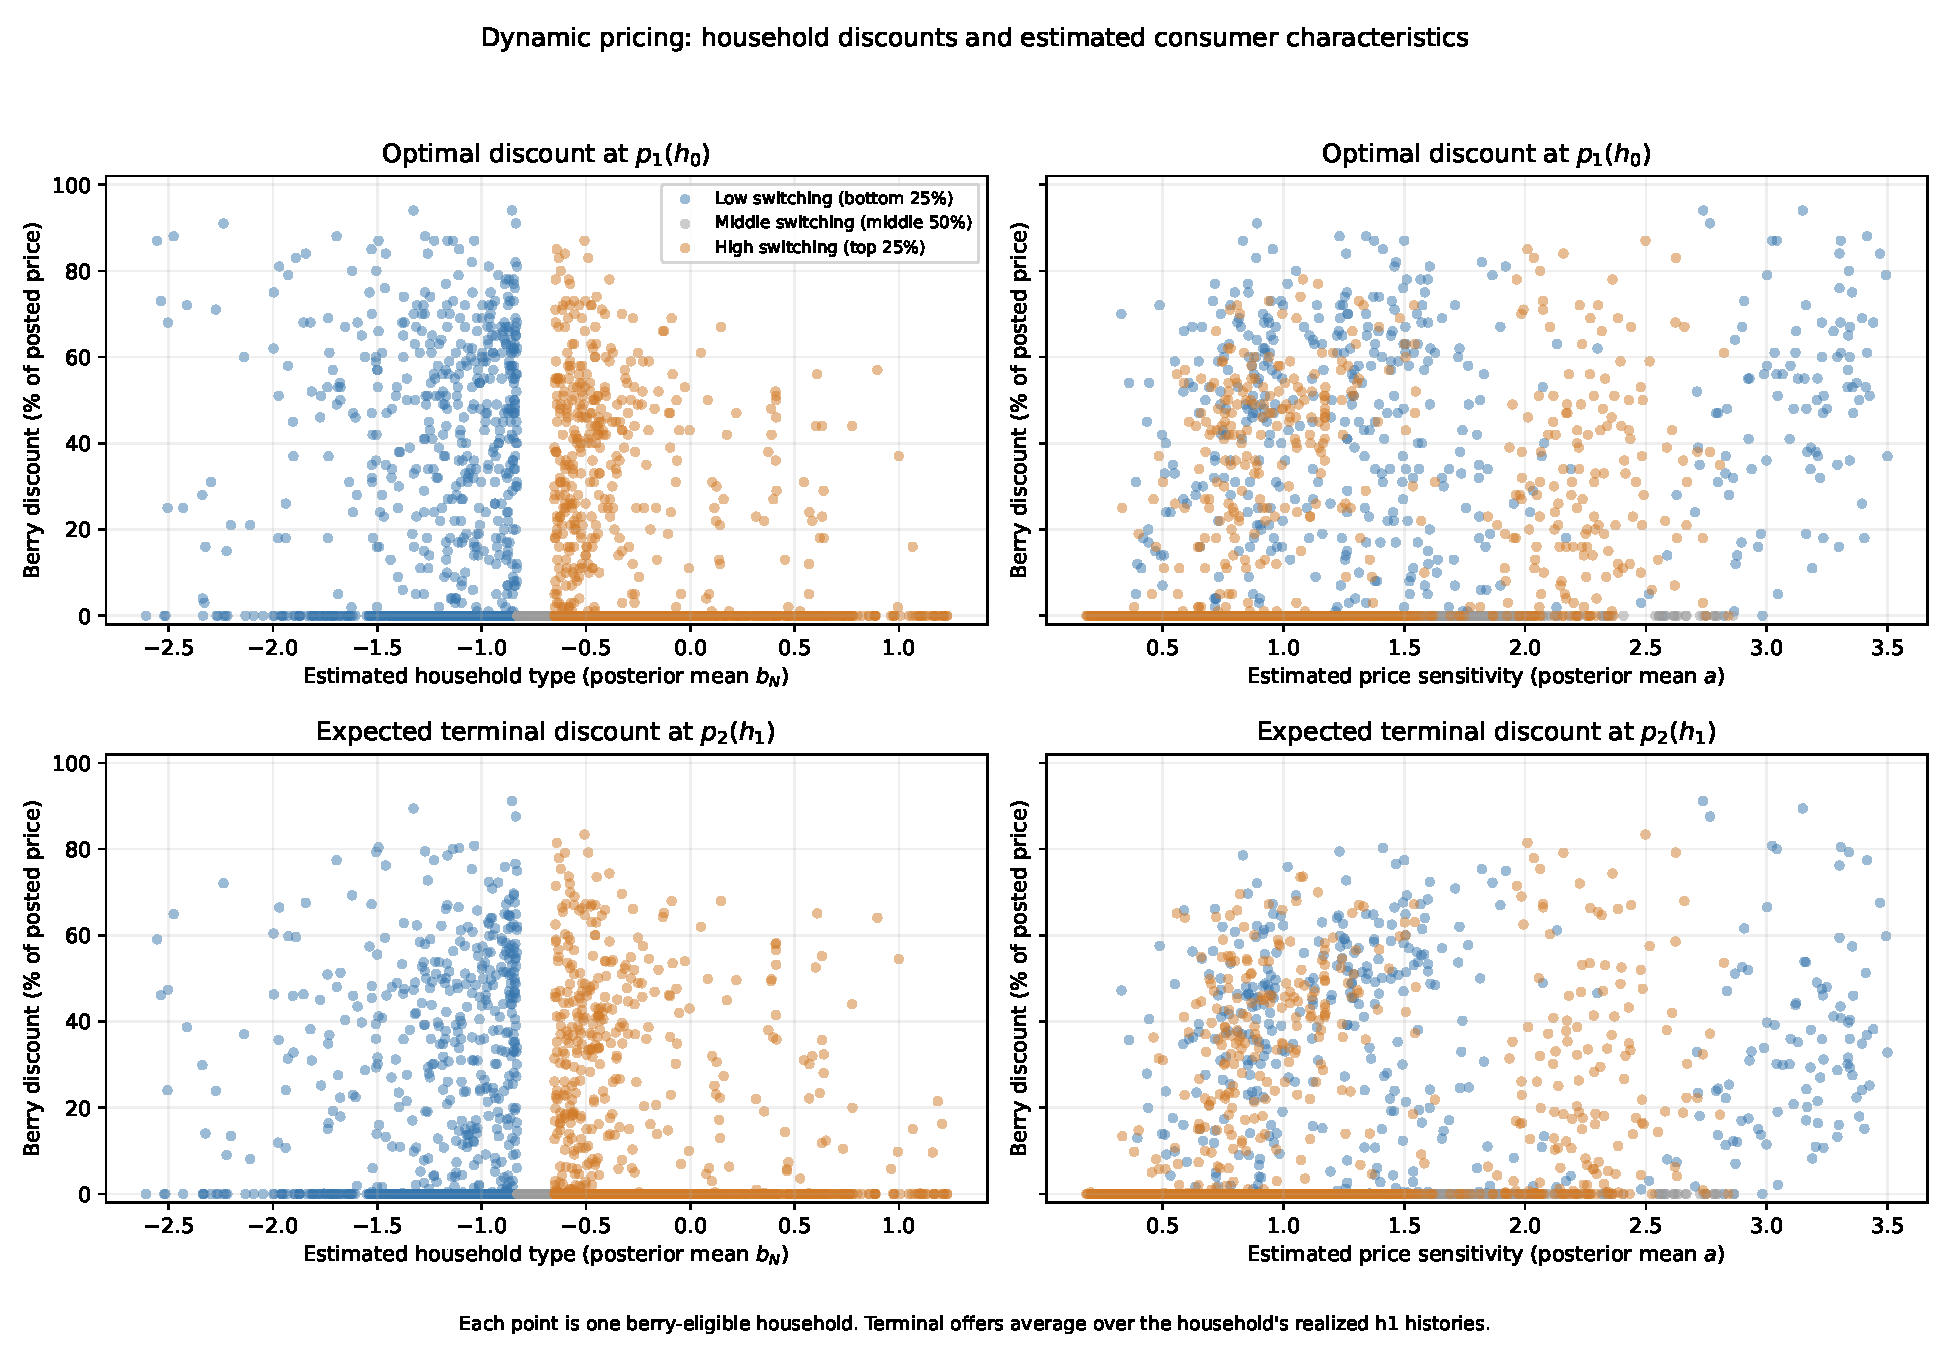
\includegraphics[width=\linewidth,height=.65\textheight,keepaspectratio]{assets/results/pricing/berry/discounts_by_household_type.pdf}
\caption{Berry: offers by household type}
\label{fig:household-type-berry}
\end{figure}
\FloatBarrier
\begin{figure}[htbp]
\centering
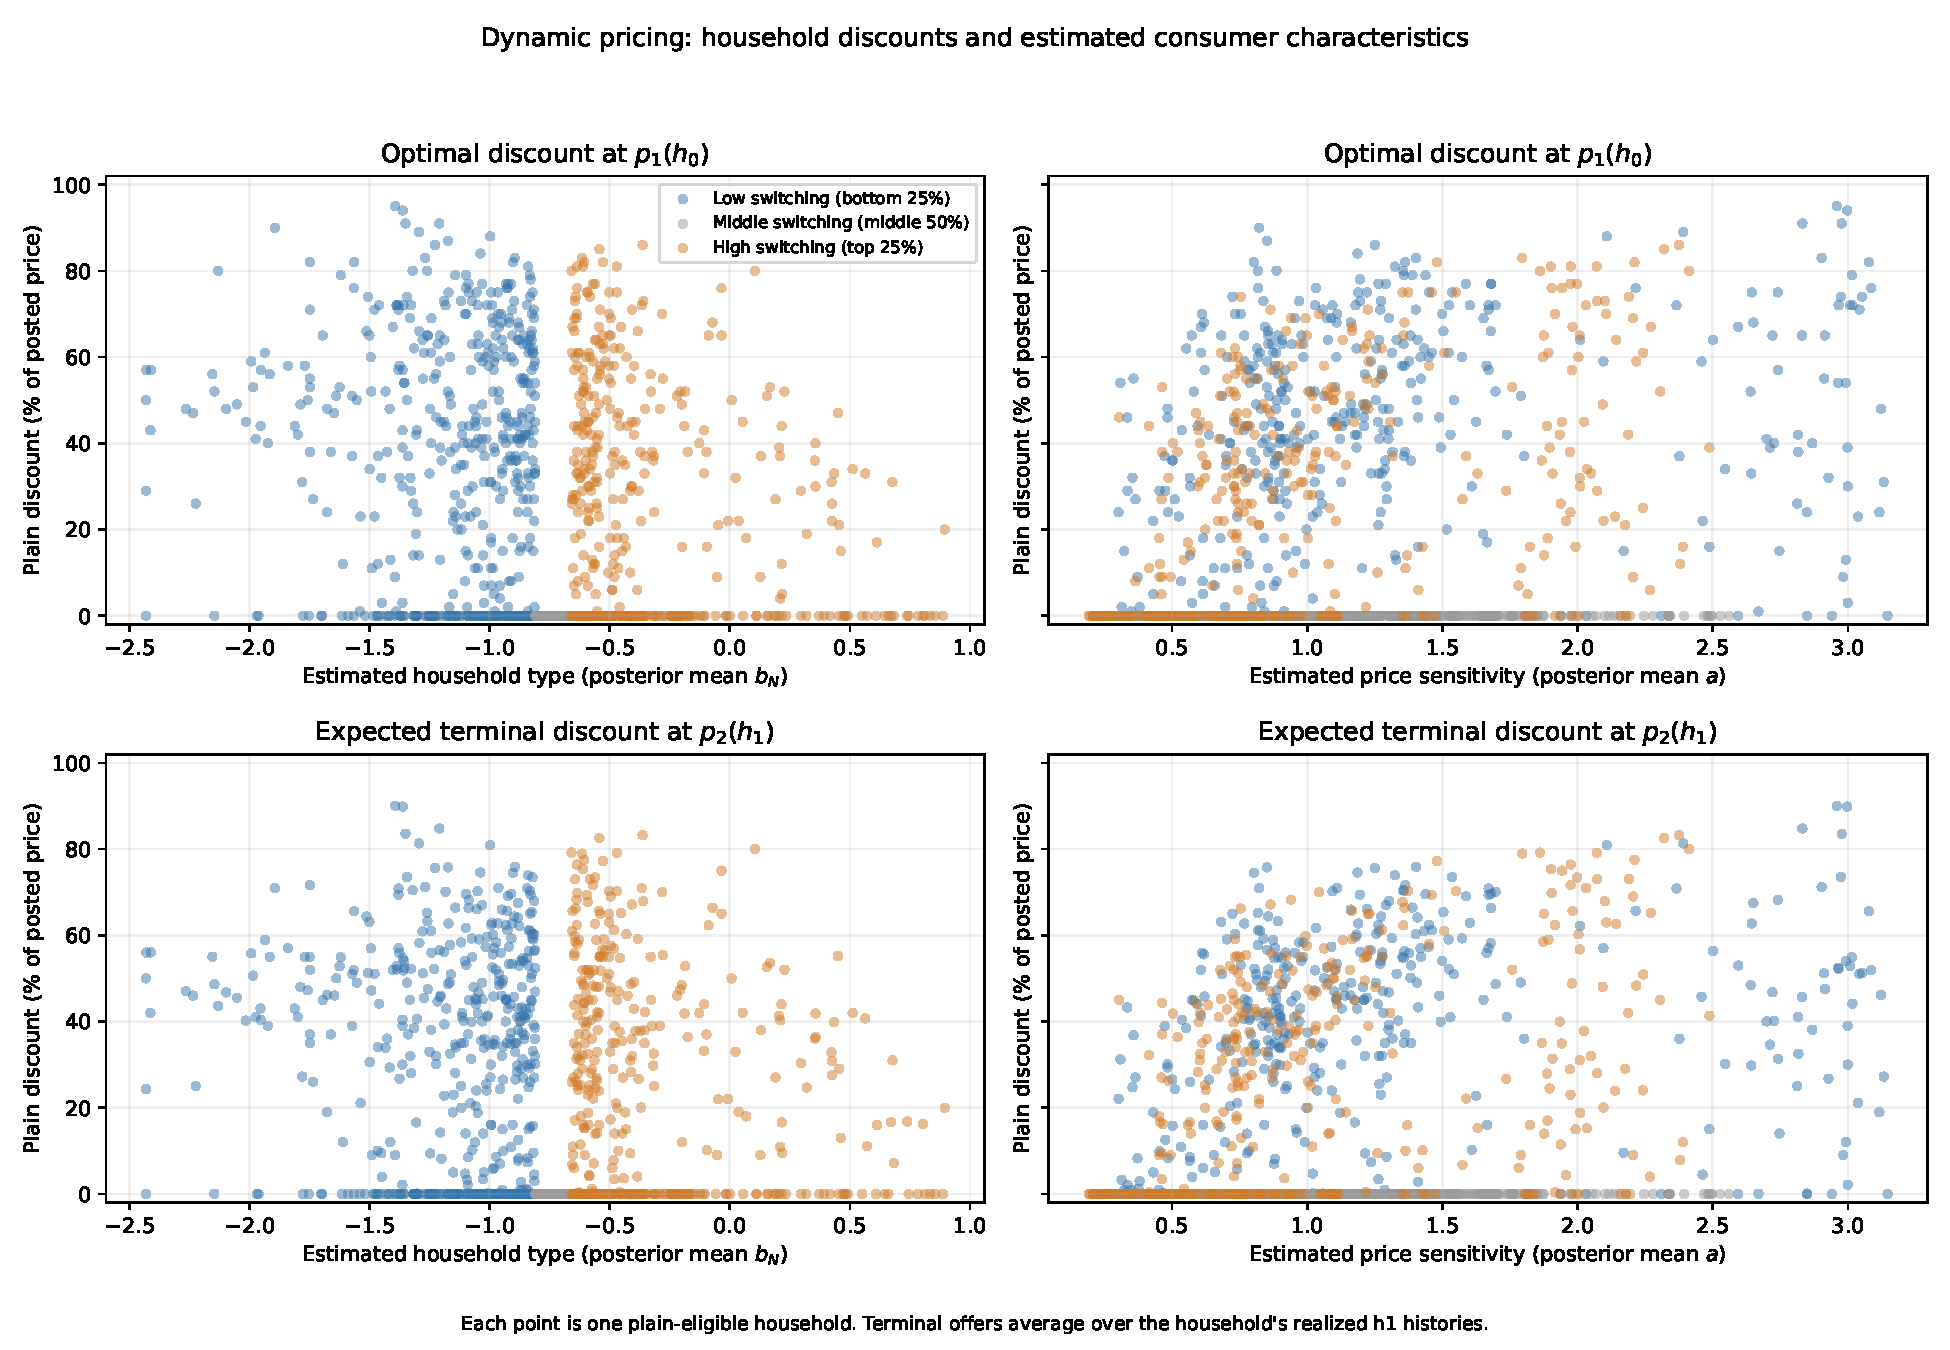
\includegraphics[width=\linewidth,height=.65\textheight,keepaspectratio]{assets/results/pricing/plain/discounts_by_household_type.pdf}
\caption{Plain: offers by household type}
\label{fig:household-type-plain}
\end{figure}
\FloatBarrier



\end{document}
